\documentclass[11pt]{article}

% -------------------- Page & Layout --------------------
\usepackage[margin=1in]{geometry}

% -------------------- Math Packages --------------------
\usepackage{amsmath, amssymb, amsthm}
\usepackage{mathtools}

% -------------------- Graphics & Figures --------------------
\usepackage{tikz}

\usepackage{graphicx}
\usepackage{pgfplots}
\pgfplotsset{compat=1.18}

% -------------------- Tables --------------------
\usepackage{array}
\usepackage{booktabs}

% -------------------- Misc --------------------
\usepackage{enumitem}   % better control of lists
\usepackage[colorlinks=true,linkcolor=blue,citecolor=blue,urlcolor=blue]{hyperref}
\usepackage[ruled,vlined]{algorithm2e}  % for algorithm environment

% -------------------- Theorem Styles --------------------
\newtheoremstyle{spaced}%
  {10pt}   % Space above
  {10pt}   % Space below
  {\itshape} % Body font
  {}       % Indent amount
  {\bfseries} % Theorem head font
  {.}      % Punctuation after theorem head
  {0.5em}  % Spa ce after theorem head
  {}       % Theorem head spec

\theoremstyle{spaced}
\newtheorem{theorem}{Theorem}[section]
\newtheorem{lemma}[theorem]{Lemma}
\newtheorem{proposition}[theorem]{Proposition}
\newtheorem{corollary}[theorem]{Corollary}

\theoremstyle{definition}
\newtheorem{definition}[theorem]{Definition}

\theoremstyle{remark}
\newtheorem{remark}[theorem]{Remark}
\newtheorem{example}[theorem]{Example}

% -------------------- Title Info --------------------
\title{Track Layouts, Forbidden Patterns, and Degree Bounds}
\author{Axel Fridman}

% =====================================================
\begin{document}
% =====================================================

\maketitle

\begin{abstract}
We study ordered layouts of a graph on $k$ ``tracks'' in which edges are 
constrained by nearest-neighbor rules. This notion comes from the Investigathon
formulation in terms of forbidden colored patterns on triples of vertices.
We make the correspondence between the two formalisms precise, define
\emph{$k$-track triplet-legal layouts}, and then investigate how many tracks
(i.e., ``colors'') are necessary for a given graph. We prove degree bounds,
planarity results for $k \le 2$, and structural examples such as cycles and
graphs obtained from a path by adding one extra edge. Along the way we
highlight exactly when $k<=2$ (``less than three colors'') is possible.
\end{abstract}

\tableofcontents

% =====================================================
\section{Basic Setup: Tracks, Order, and Legal Neighbors}
% =====================================================
\label{sec:basic-setup}
Throughout, $G=(V,E)$ is a finite simple undirected graph.

\subsection{Ordered $k$-track layouts}

We begin with the purely combinatorial structure of tracks and a global order.

\begin{definition}[Ordered $k$-track layout]
Let $k\in\mathbb{N}$. A \emph{$k$-track ordered layout} of a graph $G=(V,E)$ is a pair
\[
  (\tau,p)
\]
consisting of
\begin{itemize}[leftmargin=2em]
  \item a \emph{track assignment}
  \[
    \tau : V \to \{1,\dots,k\},
  \]
  \item and a bijective \emph{position map}
  \[
    p : V \to \{1,\dots,|V|\}.
  \]
\end{itemize}
We write $x<y$ if and only if $p(x) < p(y)$ and think of all vertices laid out
from left to right according to $p$.
\end{definition} 
An example is shown in Figure~\ref{fig:tracks-basic}.
\begin{figure}[ht]
  \centering
  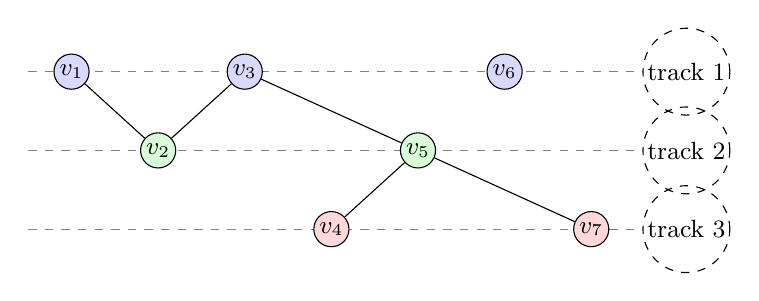
\begin{tikzpicture}[x=1.1cm,y=1cm,
    every node/.style={circle,draw,inner sep=1pt,font=\small}]
    % Track lines
    \foreach \t/\y in {1/2.0,2/1.0,3/0.0} {
      \draw[dashed,gray] (0.5,\y) -- (7.5,\y)
        node[right=1mm,black] {$\text{track }\t$};
    }

    % Vertices in global order (p(v_i) = i)
    \node[fill=blue!15]  (v1) at (1,2.0) {$v_1$};
    \node[fill=green!15] (v2) at (2,1.0) {$v_2$};
    \node[fill=blue!15]  (v3) at (3,2.0) {$v_3$};
    \node[fill=red!15]   (v4) at (4,0.0) {$v_4$};
    \node[fill=green!15] (v5) at (5,1.0) {$v_5$};
    \node[fill=blue!15]  (v6) at (6,2.0) {$v_6$};
    \node[fill=red!15]   (v7) at (7,0.0) {$v_7$};

    % Sample edges
    \draw (v1) -- (v2);
    \draw (v2) -- (v3);
    \draw (v3) -- (v5);
    \draw (v4) -- (v5);
    \draw (v5) -- (v7);
  \end{tikzpicture}
  \caption{An example of a $3$-track ordered layout: global order is left-to-right, colors indicate the track assignment $\tau$.}
  \label{fig:tracks-basic}
\end{figure}

For each track $t\in\{1,\dots,k\}$ we define the vertex set
\[
  V_t := \{v\in V : \tau(v) = t\},
\]
ordered by increasing $p(\cdot)$ along that track.

\begin{definition}[Predecessor, successor on a track]
Given a $k$-track layout $(\tau,p)$, a vertex $v\in V$, and a track $t$,
we define:
\begin{align*}
  \operatorname{pred}_t(v) 
  &:= \text{the vertex in $V_t$ with largest $p(\cdot)$ strictly less than $p(v)$ (if it exists)},\\
  \operatorname{succ}_t(v) 
  &:= \text{the vertex in $V_t$ with smallest $p(\cdot)$ strictly greater than $p(v)$ (if it exists)}.
\end{align*}
If such a vertex does not exist, the predecessor/successor is said to be
``nonexistent.'' Intuitively, these are the nearest neighbors of $v$ on track $t$
to the left/right in the global order.
\end{definition} 
See Figure~\ref{fig:predsucc} for a pictorial view along a single track.
\par\vspace{1em}


\begin{figure}[ht]
  \centering
  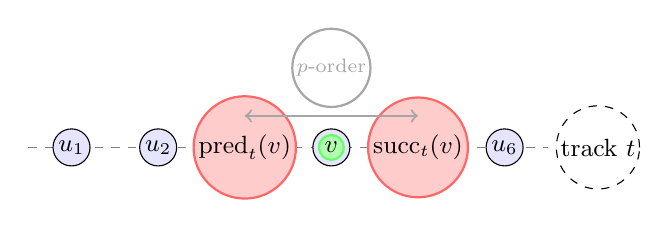
\begin{tikzpicture}[x=1.1cm,y=1cm,
    every node/.style={circle,draw,inner sep=1pt,font=\small}]
    % Single track line
    \draw[dashed,gray] (0.5,0) -- (6.5,0)
      node[right=1mm,black] {$\text{track }t$};

    % Vertices on track t
    \foreach \i in {1,...,6} {
      \node[fill=blue!10] (u\i) at (\i,0) {$u_{\i}$};
    }

    % Highlight v = u4
    \node[fill=green!30,draw=green!60,thick] (v) at (4,0) {$v$};

    % Overwrite labels for pred and succ
    \node[fill=red!20,draw=red!60,thick] (pred) at (3,0)
      {$\operatorname{pred}_t(v)$};
    \node[fill=red!20,draw=red!60,thick] (succ) at (5,0)
      {$\operatorname{succ}_t(v)$};

    % Order indication
    \draw[<->,thick,gray!70] (3,0.4) -- node[above=1mm,font=\scriptsize]
      {$p$-order} (5,0.4);
  \end{tikzpicture}
  \caption{Predecessor and successor of a vertex $v$ on a single track $t$ in the global order.}
  \label{fig:predsucc}
\end{figure}


\begin{definition}[Legal neighbor set and host graph]
Given $(\tau,p)$, the \emph{legal neighbor set} of $v\in V$ is
\[
  N_{\mathrm{legal}}(v)
  :=
  \bigl\{\operatorname{pred}_t(v), \operatorname{succ}_t(v)
        : t=1,\dots,k\bigr\}\setminus\{\text{nonexistent}\}.
\]
The corresponding \emph{host graph} $H(\tau,p)$ on vertex set $V$ has edge set
\[
  E\bigl(H(\tau,p)\bigr)
  :=
  \bigl\{\{u,v\} : u\in N_{\mathrm{legal}}(v)\bigr\}.
\]
\end{definition}
Figure~\ref{fig:legal-neighbors} shows $N_{\mathrm{legal}}(v)$ on three tracks.

\begin{figure}[ht]
  \centering
  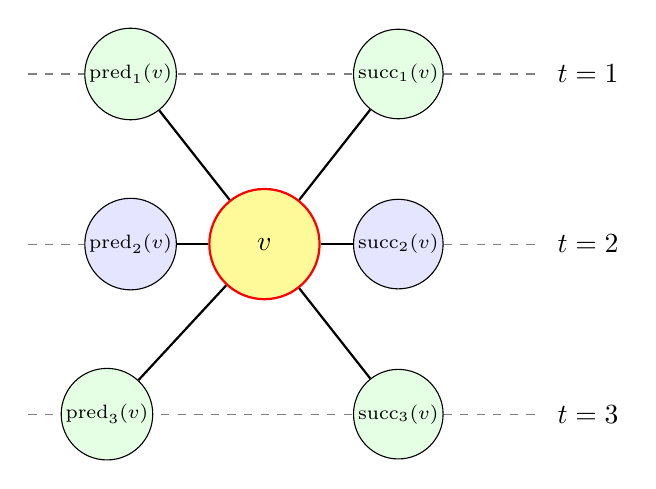
\begin{tikzpicture}[x=1.0cm,y=1.2cm,  % increased vertical spacing
    neighbor/.style={
      circle,draw,
      minimum size=10mm,  % smaller nodes
      font=\scriptsize,
      inner sep=1pt
    },
    central/.style={
      circle,draw,
      minimum size=14mm,  % central node larger
      font=\normalsize,
      inner sep=2pt,
      fill=yellow!40,
      draw=red,
      thick
    }
  ]

    % Track lines (shift y more apart so circles don't touch)
    \foreach \t/\y in {1/1.8,2/0.0,3/-1.8} {
      \draw[dashed,gray] (0.5,\y) -- (7.0,\y)
        node[right=1mm,black] {$t=\t$};
    }

    % Central vertex v
    \node[central] (v) at (3.5,0.0) {$v$};

    % Track 1 neighbors
    \node[neighbor,fill=green!10] (p1) at (1.8,1.8)
      {$\operatorname{pred}_1(v)$};
    \node[neighbor,fill=green!10] (s1) at (5.2,1.8)
      {$\operatorname{succ}_1(v)$};

    % Track 2 neighbors
    \node[neighbor,fill=blue!10] (p2) at (1.8,0.0)
      {$\operatorname{pred}_2(v)$};
    \node[neighbor,fill=blue!10] (s2) at (5.2,0.0)
      {$\operatorname{succ}_2(v)$};

    % Track 3 neighbors
    \node[neighbor,fill=green!10] (p3) at (1.5,-1.8)
      {$\operatorname{pred}_3(v)$};
    \node[neighbor,fill=green!10] (s3) at (5.2,-1.8)
      {$\operatorname{succ}_3(v)$};

    % Edges
    \foreach \w in {p1,s1,p2,s2,p3,s3} {
      \draw[thick] (v) -- (\w);
    }

  \end{tikzpicture}
  \caption{The legal neighbor set $N_{\mathrm{legal}}(v)$.}
  \label{fig:legal-neighbors}

\end{figure}



\begin{definition}[$k$-track nearest-neighbor representable graph]
A graph $G=(V,E)$ is \emph{$k$-track nearest-neighbor representable} if there
exists a $k$-track ordered layout $(\tau,p)$ of $V$ such that
\[
  E \subseteq E\bigl(H(\tau,p)\bigr),
\]
i.e.\ every edge of $G$ is a legal edge in the host graph. Equivalently,
\[
  \forall v\in V,\quad N_G(v) \subseteq N_{\mathrm{legal}}(v).
\]
The smallest such $k$ (if it exists) is the \emph{nearest-neighbor track number}
of $G$.
\end{definition}
Figure~\ref{fig:k1-linear-forest} illustrates a typical host graph when $k=1$. Figure~\ref{fig:k2-host-example} shows a typical host graph when $k=2$.


\begin{figure}[ht]
  \centering
  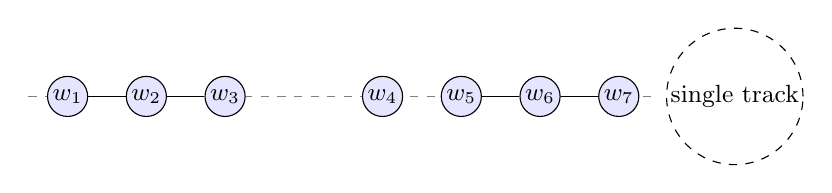
\begin{tikzpicture}[x=1cm,y=1cm,
    every node/.style={circle,draw,inner sep=1pt,font=\small}]
    % Single track
    \draw[dashed,gray] (0.5,0) -- (8.5,0)
      node[right=1mm,black] {$\text{single track}$};

    % Vertices in global order
    \foreach \i/\x in {1/1,2/2,3/3,4/5,5/6,6/7,7/8} {
      \node[fill=blue!10] (w\i) at (\x,0) {$w_{\i}$};
    }

    % Path components: w1-w2-w3 and w5-w6-w7; w4 isolated
    \draw (w1) -- (w2) -- (w3);
    \draw (w5) -- (w6) -- (w7);
  \end{tikzpicture}
  \caption{With a single track, the host graph is a disjoint union of paths and isolated vertices (a linear forest).}
  \label{fig:k1-linear-forest}
\end{figure}

\begin{figure}[ht]
  \centering
  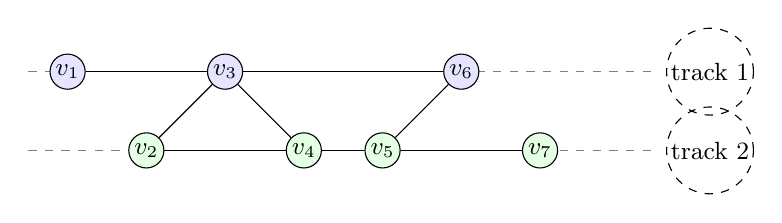
\begin{tikzpicture}[x=1cm,y=1cm,
    every node/.style={circle,draw,inner sep=1pt,font=\small}]
    % Two tracks
    \draw[dashed,gray] (0.5,1) -- (8.5,1)
      node[right=1mm,black] {$\text{track }1$};
    \draw[dashed,gray] (0.5,0) -- (8.5,0)
      node[right=1mm,black] {$\text{track }2$};

    % Vertices in global order v1,...,v7
    % Track 1: v1, v3, v6
    \node[fill=blue!10]  (v1) at (1,1) {$v_1$};
    \node[fill=blue!10]  (v3) at (3,1) {$v_3$};
    \node[fill=blue!10]  (v6) at (6,1) {$v_6$};

    % Track 2: v2, v4, v5, v7
    \node[fill=green!10] (v2) at (2,0) {$v_2$};
    \node[fill=green!10] (v4) at (4,0) {$v_4$};
    \node[fill=green!10] (v5) at (5,0) {$v_5$};
    \node[fill=green!10] (v7) at (7,0) {$v_7$};

    % Same-track edges: nearest neighbors along each track
    % Track 1 path
    \draw (v1) -- (v3) -- (v6);
    % Track 2 path
    \draw (v2) -- (v4) -- (v5) -- (v7);

    % Cross-track edges between nearest opposite-track neighbors
    \draw (v3) -- (v2);
    \draw (v3) -- (v4);
    \draw (v5) -- (v6);

  \end{tikzpicture}
  \caption{With two tracks, the host graph may have path-like pieces on each track plus cross-track edges between nearest neighbors on the other track.}
  \label{fig:k2-host-example}
\end{figure}


\begin{remark}[What $k=1$ really means]
\label{rem:what-k1-means}
When $k=1$, every vertex has at most one predecessor and one successor,
so the host graph $H(\tau,p)$ is a subgraph of a simple path. Thus any
$1$-track nearest-neighbor representable graph is a disjoint union of paths
and isolated vertices (a \emph{linear forest}). This will be important when
we discuss whether ``less than two colors'' (tracks) is possible.
\end{remark}

\begin{remark}[What $k=2$ really means]
\label{rem:what-k2-means}

When $k=2$, each vertex can have at most two legal neighbors on its own track
(one predecessor and one successor) and at most two legal neighbors on the
other track (again, one predecessor and one successor there). Thus every
vertex in the host graph $H(\tau,p)$ has degree at most $4$, and $H(\tau,p)$
can be viewed as two path-like layers (one per track) with additional
nearest-neighbor cross edges between the layers, as in
Figure~\ref{fig:k2-host-example}. In particular, any $2$-track
nearest-neighbor representable graph is a subgraph of such a ``ladder-like''
planar host graph. This will be important when we discuss when
``less than three colors'' (tracks) is possible.
\end{remark}

% =====================================================
\section{From Forbidden Colored Patterns to Triplet Constraints}
% =====================================================

The Investigathon formulation uses forbidden \emph{colored patterns} on triples
of vertices. We now translate that language into our $k$-track layout setting.

\subsection{Colored patterns on triples}

\begin{definition}[Colored pattern on three vertices]
Fix the index set $\{1,2,3\}$. A (plain) \emph{pattern} is a pair
\[
  (E_P, N_P),
\]
where $E_P, N_P \subseteq \{1,2,3\} \times \{1,2,3\}$ encode edges that must
be present and edges that must be absent between the three distinguished
positions.

A \emph{colored pattern} is a triple
\[
  P = (E_P, N_P, C_P),
\]
where $(E_P, N_P)$ is a pattern as above and
$C_P \subseteq \{1,2,3\}$ is the set of indices that are required to lie
in the same color class.
\end{definition}

In the Investigathon setting, the input is:
\begin{itemize}[leftmargin=2em]
  \item a linear order $<$ on $V(G)$, and
  \item a partition (``coloring'')
    $\mathcal{S} = \{S_1,\dots,S_k\}$ of $V(G)$ into $k$ color classes.
\end{itemize}

\begin{definition}[Realizing a colored pattern]
Given $(\mathcal{S},<)$ as above and a colored pattern
$P = (E_P,N_P,C_P)$, an ordered triple of distinct vertices
\[
  v_1 < v_2 < v_3
\]
\emph{realizes} $P$ if:
\begin{enumerate}[label=(\roman*), leftmargin=2em]
  \item for every $(i,j)\in E_P$ we have $\{v_i,v_j\}\in E(G)$;
  \item for every $(i,j)\in N_P$ we have $\{v_i,v_j\}\notin E(G)$;
  \item all $v_i$ with $i\in C_P$ lie in a common color class in $\mathcal{S}$.
\end{enumerate}
We say that $(\mathcal{S},<)$ \emph{avoids} $P$ if no triple $v_1<v_2<v_3$
realizes $P$.
\end{definition}

Given a finite family $\Pi$ of colored patterns, $(\mathcal{S},<)$ \emph{avoids
$\Pi$} if it avoids every $P\in\Pi$.

\subsection{The Investigathon patterns}

In our case, the forbidden family $\Pi$ consists of the two patterns
\begin{align*}
  P^{(1)} &: \quad
    E_{P^{(1)}} = \{(1,3)\},\quad
    N_{P^{(1)}} = \varnothing,\quad
    C_{P^{(1)}} = \{1,2\},\\[0.3em]
  P^{(2)} &: \quad
    E_{P^{(2)}} = \{(1,3)\},\quad
    N_{P^{(2)}} = \varnothing,\quad
    C_{P^{(2)}} = \{2,3\}.
\end{align*}
Intuitively:
\begin{itemize}[leftmargin=2em]
  \item $P^{(1)}$ forbids triples $x<y<z$ with $\{x,z\}\in E(G)$ and $x,y$
        of the same color;
  \item $P^{(2)}$ forbids triples $x<y<z$ with $\{x,z\}\in E(G)$ and $y,z$
        of the same color.
\end{itemize}
See Figure~\ref{fig:pattern-P1} and ~\ref{fig:pattern-P2}.
\begin{figure}[ht]
  \centering
  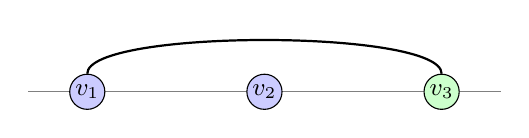
\begin{tikzpicture}[x=1.5cm,y=1cm,
    every node/.style={circle,draw,inner sep=1pt,font=\small}]
    % Order line
    \draw[gray] (0.5,0) -- (4.5,0);

    % Vertices v1 < v2 < v3
    \node[fill=blue!20]  (v1) at (1,0) {$v_1$};
    \node[fill=blue!20]  (v2) at (2.5,0) {$v_2$};
    \node[fill=green!20] (v3) at (4,0) {$v_3$};

    % Edge {v1,v3}
    \draw[thick] (v1) .. controls +(0,0.8) and +(0,0.8) .. (v3);


  \end{tikzpicture}
  \caption{Forbidden pattern $P^{(1)}$: $v_1<v_2<v_3$ with $\{v_1,v_3\}\in E(G)$ and $v_1,v_2$ in the same color class.}
  \label{fig:pattern-P1}
\end{figure}
\begin{figure}[ht]
  \centering
  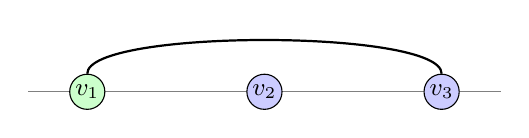
\begin{tikzpicture}[x=1.5cm,y=1cm,
    every node/.style={circle,draw,inner sep=1pt,font=\small}]
    % Order line
    \draw[gray] (0.5,0) -- (4.5,0);

    % Vertices v1 < v2 < v3
    \node[fill=green!20] (v1) at (1,0) {$v_1$};
    \node[fill=blue!20]  (v2) at (2.5,0) {$v_2$};
    \node[fill=blue!20]  (v3) at (4,0) {$v_3$};

    % Edge {v1,v3}
    \draw[thick] (v1) .. controls +(0,0.8) and +(0,0.8) .. (v3);


  \end{tikzpicture}
  \caption{Forbidden pattern $P^{(2)}$: $v_1<v_2<v_3$ with $\{v_1,v_3\}\in E(G)$ and $v_2,v_3$ in the same color class.}
  \label{fig:pattern-P2}
\end{figure}

A \emph{solution with at most $k$ colors} in the Investigathon sense is precisely
a pair $(\mathcal{S},<)$ with $|\mathcal{S}|\le k$ that avoids
$P^{(1)}$ and $P^{(2)}$.

\subsection{Tracks as color classes}

Given a $k$-track layout $(\tau,p)$, the track assignment induces a
partition into color classes
\[
  S_i := \{ v\in V(G) : \tau(v) = i \},
  \qquad \mathcal{S} = \{S_1,\dots,S_k\},
\]
and the global order $<$ is defined by $p$.

Conversely, given a partition $\mathcal{S} = \{S_1,\dots,S_k\}$ and a
linear order $<$, we obtain a $k$-track layout by labeling the parts
$S_1,\dots,S_k$ and setting $\tau(v)=i$ for $v\in S_i$, and letting
$p$ be any bijection consistent with $<$.

Thus there is a one-to-one correspondence between:
\begin{itemize}[leftmargin=2em]
  \item solutions $(\mathcal{S},<)$ with at most $k$ colors, and
  \item $k$-track ordered layouts $(\tau,p)$.
\end{itemize}

\subsection{Triplet constraint formulation}

We now restate avoidance of $P^{(1)}$ and $P^{(2)}$ in a compact way.

\begin{lemma}[Colored patterns vs.\ triplet constraint]
\label{lem:patterns-triplet-equivalence}
Let $G=(V,E)$ be a graph and let $(\tau,p)$ be a $k$-track ordered layout
with associated order $<$ and induced partition $\mathcal{S}$ as above.
Then the following are equivalent:
\begin{enumerate}[label=(\arabic*), leftmargin=2em]
  \item $(\mathcal{S},<)$ avoids both colored patterns $P^{(1)}$ and $P^{(2)}$.
  \item For every triple $x,y,z\in V$ with
        \[
          p(x) < p(y) < p(z)
          \quad\text{and}\quad
          \{x,z\}\in E(G),
        \]
        we have
        \[
          \tau(y) \neq \tau(x)
          \quad\text{and}\quad
          \tau(y) \neq \tau(z).
        \]
\end{enumerate}
\end{lemma}

\begin{proof}
$(1)\Rightarrow(2)$:
Suppose there exist $x,y,z$ with $p(x)<p(y)<p(z)$ and $\{x,z\}\in E(G)$
such that $\tau(y)=\tau(x)$ or $\tau(y)=\tau(z)$.

Write $v_1:=x$, $v_2:=y$, $v_3:=z$. Then $\{v_1,v_3\}\in E(G)$.
If $\tau(y)=\tau(x)$ then $v_1$ and $v_2$ lie in the same color class and
$(v_1,v_2,v_3)$ realizes $P^{(1)}$, contradicting avoidance of $P^{(1)}$.
If $\tau(y)=\tau(z)$ then $(v_1,v_2,v_3)$ realizes $P^{(2)}$, a contradiction.
Thus $\tau(y)$ differs from both $\tau(x)$ and $\tau(z)$.

\medskip
$(2)\Rightarrow(1)$:
Assume (2) holds. Suppose some triple $v_1<v_2<v_3$ realizes $P^{(1)}$.
Then $\{v_1,v_3\}\in E(G)$ and $v_1,v_2$ lie in the same color class, i.e.\
$\tau(v_1)=\tau(v_2)$, contradicting (2) with $(x,y,z)=(v_1,v_2,v_3)$.
An identical argument with roles of positions $\{1,2\}$ and $\{2,3\}$
exchanged shows that no triple realizes $P^{(2)}$ either.
\end{proof}

\begin{definition}[$k$-track triplet-legal layout]
A $k$-track ordered layout $(\tau,p)$ of $G$ is \emph{triplet-legal} if for
every $x,y,z\in V$ with
\[
  p(x) < p(y) < p(z) \quad\text{and}\quad \{x,z\}\in E(G),
\]
we have
\[
  \tau(y) \neq \tau(x)
  \quad\text{and}\quad
  \tau(y) \neq \tau(z).
\]
By Lemma~\ref{lem:patterns-triplet-equivalence}, triplet-legal layouts are
exactly the layouts corresponding to Investigathon solutions avoiding
$P^{(1)}$ and $P^{(2)}$.
\end{definition}
Figure~\ref{fig:triplet-legal} contrasts a forbidden and two legal triples, one using fewer colors than the other.
\begin{figure}[ht]
  \centering
  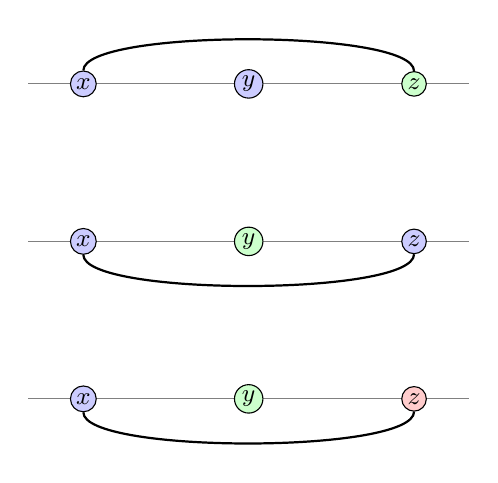
\begin{tikzpicture}[x=1.4cm,y=1cm,
    every node/.style={circle,draw,inner sep=1pt,font=\small}]

    % Forbidden triple (top)
    \draw[gray] (0.5,0.8) -- (4.5,0.8);
    \node[fill=blue!20]  (x1) at (1,0.8) {$x$};
    \node[fill=blue!20]  (y1) at (2.5,0.8) {$y$};
    \node[fill=green!20] (z1) at (4,0.8) {$z$};
    \draw[thick] (x1) .. controls +(0,0.7) and +(0,0.7) .. (z1);

    % Legal triple (bottom)
    \draw[gray] (0.5,-1.2) -- (4.5,-1.2);
    \node[fill=blue!20]  (x2) at (1,-1.2) {$x$};
    \node[fill=green!20] (y2) at (2.5,-1.2) {$y$};
    \node[fill=blue!20]   (z2) at (4,-1.2) {$z$};
    \draw[thick] (x2) .. controls +(0,-0.7) and +(0,-0.7) .. (z2);

    \draw[gray] (0.5,-3.2) -- (4.5,-3.2);
    \node[fill=blue!20]  (x3) at (1,-3.2) {$x$};
    \node[fill=green!20] (y3) at (2.5,-3.2) {$y$};
    \node[fill=red!20]   (z3) at (4,-3.2) {$z$};
    \draw[thick] (x3) .. controls +(0,-0.7) and +(0,-0.7) .. (z3);
  \end{tikzpicture}
  \caption{Top: a forbidden triple where $y$ shares a track (color) with $x$. 
  Middle: a legal triple where $x$ shares a track (color) with $z$. 
  Bottom: a legal triple where the middle vertex lies on a third track.}
  \label{fig:triplet-legal}
\end{figure}

\begin{remark}[Nearest-neighbor vs.\ triplet-legal]
Nearest-neighbor representability is a \emph{stronger} requirement than
being triplet-legal: in a nearest-neighbor layout, every edge must be
between nearest neighbors on some track; in a triplet-legal layout we
only forbid certain colored patterns on triples. In the next section we
show that nearest-neighbor layouts automatically satisfy the triplet
constraint.
\end{remark}
% =====================================================
\section{Chromatic Number vs.\ Track-Based ``Colors''}
% =====================================================

The track index $\tau(v)$ behaves a bit like a color, but it is \emph{not} a
proper graph coloring in the classical sense (edges within a track are
allowed). We only need two standard facts from ordinary graph coloring for
analogy:

\begin{itemize}[leftmargin=2em]
  \item If $G_1,\dots,G_r$ are the connected components of $G$, then
        \[
          \chi(G) \;=\; \max_{1\le i\le r} \chi(G_i).
        \]
  \item If $G$ contains a clique of size $r$, then $\chi(G)\ge r$; in
        particular a $K_4$ forces at least four colors.
\end{itemize}

In the nearest-neighbor setting, track labels play the role of “colors”, and
we will see analogues of both statements for the track number.

\subsection{Track number and connected components}

\begin{definition}[Nearest-neighbor track number]
The \emph{nearest-neighbor track number} of a graph $G$, denoted
$\operatorname{tn}(G)$, is the smallest $k\in\mathbb{N}$ for which $G$ is
$k$-track nearest-neighbor representable.
\end{definition}

\begin{proposition}[Track number and connected components]
\label{prop:tracknumber-components}
Let $G_1,\dots,G_r$ be the connected components of $G$. Then
\[
  \operatorname{tn}(G)
  \;=\;
  \max_{1\le i\le r} \operatorname{tn}(G_i).
\]
\end{proposition}
\begin{remark}
Proposition~\ref{prop:tracknumber-components} is directly analogous to the
classical fact that $\chi(G) = \max_i \chi(G_i)$ for the chromatic number:
in both settings, the number of ``colors'' needed for the whole graph is the
maximum over its connected components.
\end{remark}

\begin{proof}
\emph{Lower bound.}
Any layout witnessing $G$ as $k$-track nearest-neighbor representable
restricts to a layout for each $G_i$, so $\operatorname{tn}(G_i)\le k$.
Taking the minimum over all such $k$ gives
\(
  \max_i \operatorname{tn}(G_i) \le \operatorname{tn}(G).
\)

\smallskip
\noindent\emph{Upper bound.}
Let $k_i = \operatorname{tn}(G_i)$ and $k:=\max_i k_i$. For each component
$G_i$ choose a $k_i$-track layout $(\tau_i,p_i)$ witnessing
nearest-neighbor representability. Relabel tracks so that $\tau_i$ takes
values in $\{1,\dots,k\}$ (we simply do not use all labels when $k_i<k$).

Now place the components one after another in the global order: define $p$
by stacking the orders $p_1,\dots,p_r$ with disjoint ranges, and set
$\tau(v)=\tau_i(v)$ for $v\in V(G_i)$. This gives a $k$-track layout
$(\tau,p)$ of $G$ in which every edge inside each component remains legal.
There are no edges between components, so nothing else needs to be checked.
Hence $G$ is $k$-track nearest-neighbor representable and
$\operatorname{tn}(G)\le k$.
\end{proof}

Figure~\ref{fig:tn-components} shows how track layouts for components can be
stacked in the global order while reusing the same set of track labels.

\begin{figure}[ht]
  \centering
  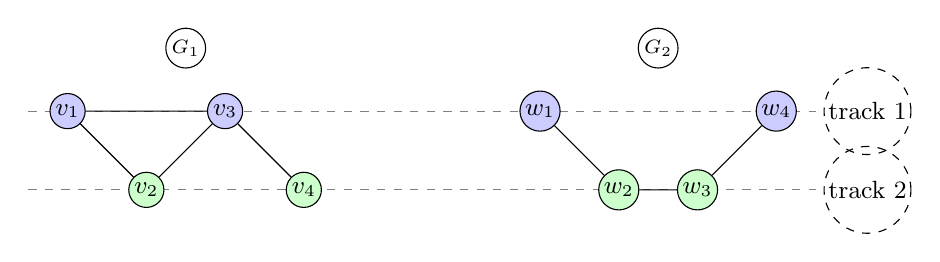
\begin{tikzpicture}[x=1.0cm,y=1cm,
    every node/.style={circle,draw,inner sep=1pt,font=\small}]

    % Track lines
    \foreach \t/\y in {1/1.0,2/0.0} {
      \draw[dashed,gray] (0.5,\y) -- (10.5,\y)
        node[right=1mm,black] {$\text{track }\t$};
    }

    % Component G1 on the left (vertices v1..v4)
    \node[fill=blue!20] (v1) at (1,1.0) {$v_1$};
    \node[fill=green!20] (v2) at (2,0.0) {$v_2$};
    \node[fill=blue!20] (v3) at (3,1.0) {$v_3$};
    \node[fill=green!20] (v4) at (4,0.0) {$v_4$};
    \draw (v1) -- (v2) -- (v3) -- (v4) -- (v3) -- (v1);

    % Component G2 on the right (vertices w1..w4)
    \node[fill=blue!20] (w1) at (7,1.0) {$w_1$};
    \node[fill=green!20] (w2) at (8,0.0) {$w_2$};
    \node[fill=green!20] (w3) at (9,0.0) {$w_3$};
    \node[fill=blue!20] (w4) at (10,1.0) {$w_4$};
    \draw (w1) -- (w2) -- (w3) -- (w4);

    \node at (2.5,1.8) {\scriptsize $G_1$};
    \node at (8.5,1.8) {\scriptsize $G_2$};
  \end{tikzpicture}
  \caption{Layouts for different components share the same track labels.
  The global order stacks the components one after another.}
  \label{fig:tn-components}
\end{figure}

\begin{remark}[When is fewer than $2$ tracks enough?]
From Section~\ref{sec:basic-setup}, a $1$-track host graph is always a
disjoint union of paths and isolated vertices (a linear forest). Thus
\[
  \operatorname{tn}(G)=1 \quad\Longleftrightarrow\quad
  G \text{ is a linear forest},
\]
and any graph containing a cycle requires at least two tracks. Figure
\ref{fig:cycle-needs-two} illustrates why a cycle cannot live on a single
track.
\end{remark}

\begin{figure}[ht]
  \centering
  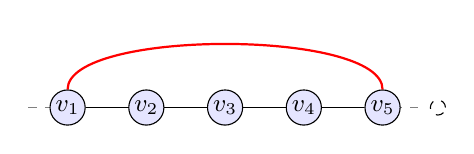
\begin{tikzpicture}[x=1cm,y=1cm,
    every node/.style={circle,draw,inner sep=1pt,font=\small}]

    % Single track
    \draw[dashed,gray] (0.5,0) -- (5.5,0)
      node[right=1mm,black] {$\text{ }$};

    % Vertices in order v1..v5
    \foreach \i/\x in {1/1,2/2,3/3,4/4,5/5} {
      \node[fill=blue!10] (v\i) at (\x,0) {$v_{\i}$};
    }

    % Path edges (legal)
    \draw (v1) -- (v2) -- (v3) -- (v4) -- (v5);

    % Extra edge v5-v1 (would form a cycle)
    \draw[thick,red] (v1) .. controls +(0,1) and +(0,1) .. (v5);

  \end{tikzpicture}
  \caption{On a single track, only edges between consecutive vertices can be
  legal. The edge $\{v_1,v_5\}$ needed to complete a cycle skips three
  vertices and cannot be realized.}
  \label{fig:cycle-needs-two}
\end{figure}

% =====================================================
\section{Nearest-Neighbor Layouts Satisfy the Triplet Constraint}
% =====================================================

We now connect the nearest-neighbor condition back to the triplet constraint
of Lemma~\ref{lem:patterns-triplet-equivalence}.

\begin{lemma}[Triplet constraint for nearest-neighbor layouts]
\label{lem:triplet}
Let $(\tau,p)$ be a $k$-track ordered layout of a graph $G=(V,E)$ and suppose
that $G$ is $k$-track nearest-neighbor representable with respect to $(\tau,p)$,
i.e.
\[
  N_G(v) \subseteq N_{\mathrm{legal}}(v)
  \quad\text{for all }v\in V.
\]
Let $x,y,z\in V$ such that
\[
  p(x) < p(y) < p(z),
\]
and suppose $\{x,z\}\in E$. Then
\[
  \tau(y) \neq \tau(x)
  \quad\text{and}\quad
  \tau(y) \neq \tau(z).
\]
In words: any vertex strictly between adjacent vertices $x$ and $z$ in the
global order must lie on a track different from both $\tau(x)$ and $\tau(z)$.
\end{lemma}
Figure~\ref{fig:triplet-lemma} shows the situation in Lemma~\ref{lem:triplet}.

\begin{figure}[ht]
  \centering
  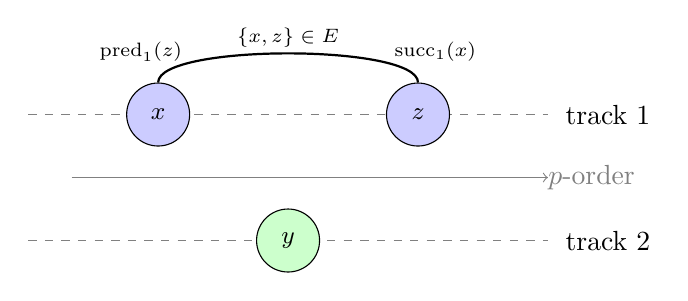
\begin{tikzpicture}[
    x=1.1cm,y=1cm,
    vertex/.style={circle,draw,inner sep=1pt,minimum size=8mm,font=\small}
  ]

    % Two tracks
    \draw[dashed,gray] (0.5,0.8) -- (6.5,0.8)
      node[right=1mm,black] {$\text{track }1$};
    \draw[dashed,gray] (0.5,-0.8) -- (6.5,-0.8)
      node[right=1mm,black] {$\text{track }2$};

    % x and z on track 1, y on track 2 (bigger vertices)
    \node[vertex,fill=blue!20] (x) at (2,0.8) {$x$};
    \node[vertex,fill=blue!20] (z) at (5,0.8) {$z$};
    \node[vertex,fill=green!20] (y) at (3.5,-0.8) {$y$};

    % Global order on the x-axis
    \draw[->,gray] (1,0) -- (6.5,0)
      node[right,draw=none,inner sep=0] {$p$-order};

    % Edge between x and z
    \draw[thick] (x) .. controls +(0,0.9) and +(0,0.9) .. (z);
    \node[above=7mm,draw=none,inner sep=0] at (3.5,0.95)
      {\scriptsize $\{x,z\}\in E$};

    % Nearest neighbors of x and z on track 1 (no circles)
    \node[draw=none,inner sep=0,font=\scriptsize] at (1.8,1.6)
      {$\operatorname{pred}_1(z)$};
    \node[draw=none,inner sep=0,font=\scriptsize] at (5.2,1.6)
      {$\operatorname{succ}_1(x)$};

  \end{tikzpicture}
  \caption{If $\{x,z\}$ is an edge coming from nearest neighbors on track~1, then no other vertex on track~1 can lie between them in the global order. Hence any middle vertex $y$ must live on a different track.}
  \label{fig:triplet-lemma}
\end{figure}


\begin{proof}
Since $\{x,z\}\in E$ and $G$ is nearest-neighbor representable, we have
\[
  z \in N_{\mathrm{legal}}(x)
  \quad\text{and}\quad
  x \in N_{\mathrm{legal}}(z).
\]

\medskip
\noindent\emph{Step 1: $z$ is the successor of $x$ on track $\tau(z)$.}

By definition of $N_{\mathrm{legal}}(x)$, there exists a track $t$ such that
\[
  z = \operatorname{pred}_t(x)
  \quad\text{or}\quad
  z = \operatorname{succ}_t(x).
\]
If $z = \operatorname{pred}_t(x)$ then $p(z)<p(x)$, contradicting
$p(x)<p(z)$; hence
\[
  z = \operatorname{succ}_t(x).
\]
Moreover, $\operatorname{succ}_t(x)$ lies on track $t$, hence
$\tau(z)=t$ and
\[
  z = \operatorname{succ}_{\tau(z)}(x).
\]

By definition of successor, there is no vertex $w$ on track $\tau(z)$
with global position strictly between $p(x)$ and $p(z)$, i.e.
\[
  \text{no }w\text{ satisfies }\tau(w)=\tau(z)\text{ and }p(x)<p(w)<p(z).
\]
Since $p(x)<p(y)<p(z)$, we cannot have $\tau(y)=\tau(z)$.

\medskip
\noindent\emph{Step 2: $x$ is the predecessor of $z$ on track $\tau(x)$.}

Similarly, since $x\in N_{\mathrm{legal}}(z)$ there exists some track $s$
such that
\[
  x = \operatorname{pred}_s(z)
  \quad\text{or}\quad
  x = \operatorname{succ}_s(z).
\]
Because $p(x)<p(z)$, $x$ cannot be a successor of $z$, so
\[
  x = \operatorname{pred}_s(z).
\]
Hence $\tau(x)=s$ and
\[
  x = \operatorname{pred}_{\tau(x)}(z).
\]
Again by definition of predecessor, there is no vertex $w$ on track $\tau(x)$
with $p(x)<p(w)<p(z)$. In particular, $\tau(y)\neq \tau(x)$.

\medskip
Combining both steps, we obtain $\tau(y)\neq\tau(x)$ and
$\tau(y)\neq\tau(z)$.
\end{proof}

\begin{corollary}
Every $k$-track nearest-neighbor layout $(\tau,p)$ is a $k$-track triplet-legal
layout. In particular, any nearest-neighbor solution automatically avoids the
Investigathon patterns $P^{(1)}$ and $P^{(2)}$.
\end{corollary}

\begin{proof}
Apply Lemma~\ref{lem:triplet} and then use
Lemma~\ref{lem:patterns-triplet-equivalence}.
\end{proof}

% =====================================================
\section{Degree Bounds and Clique Constraints}
% =====================================================

We now quantify how the number of tracks $k$ controls the possible degrees
and cliques in a nearest-neighbor representable graph. This addresses
one natural way to \emph{lower-bound} the number of ``colors'' (tracks)
required.

\subsection{A $K_4$ forces at least three tracks}

\begin{theorem}[A $4$-clique forces $k\ge 3$]
\label{thm:K4-needs-3}
Let $G=(V,E)$ be a graph that is $k$-track nearest-neighbor representable
for some $k\in\mathbb{N}$. If $G$ contains a clique of size $4$, then
$k \ge 3$. Equivalently, no $1$- or $2$-track layout can represent a $4$-clique.
\end{theorem}

\begin{proof}
Let $H\subseteq G$ be a subgraph isomorphic to $K_4$ with vertex set
$\{a,b,c,d\}$. Let $(\tau,p)$ be a $k$-track ordered layout witnessing
nearest-neighbor representability of $G$.

Rename $a,b,c,d$ so that
\[
  p(a) < p(b) < p(c) < p(d).
\]
Since $H$ is complete, every pair among $\{a,b,c,d\}$ is an edge.

Using Lemma~\ref{lem:triplet}, we apply the triplet constraint to all
triples $(x,y,z)$ with $x<y<z$ where $\{x,z\}$ is an edge (always true in
$K_4$). The relevant triples and consequences are:
\begin{align}
\tau(b) &\neq \tau(a), \quad \tau(b) \neq \tau(c),
   &&\text{from }(a,b,c)\text{ and edge }\{a,c\}, \label{eq:bc1}\\
\tau(b) &\neq \tau(a), \quad \tau(b) \neq \tau(d),
   &&\text{from }(a,b,d)\text{ and edge }\{a,d\}, \label{eq:bd1}\\
\tau(c) &\neq \tau(a), \quad \tau(c) \neq \tau(d),
   &&\text{from }(a,c,d)\text{ and edge }\{a,d\}, \label{eq:cd1}\\
\tau(c) &\neq \tau(b), \quad \tau(c) \neq \tau(d),
   &&\text{from }(b,c,d)\text{ and edge }\{b,d\}. \label{eq:cd2}
\end{align}
From \eqref{eq:bc1} and \eqref{eq:bd1} we see that
\[
  \tau(b) \notin \{\tau(a),\tau(c),\tau(d)\},
\]
and from \eqref{eq:cd1} and \eqref{eq:cd2} that
\[
  \tau(c) \notin \{\tau(a),\tau(b),\tau(d)\}.
\]

Suppose $k\le 2$. Then tracks are $\{1,2\}$.
Without loss of generality, let $\tau(a)=1$.

\smallskip
\noindent\emph{Case 1: $\tau(d)=1$.}
Then \eqref{eq:bd1} implies $\tau(b)\neq \tau(a)$ and $\tau(b)\neq \tau(d)$,
so $\tau(b)\neq 1$ and hence $\tau(b)=2$. Similarly, \eqref{eq:cd1} implies
$\tau(c)\neq 1$, so $\tau(c)=2$. But then \eqref{eq:bc1} requires
$\tau(b)\neq \tau(c)$, impossible.

\smallskip
\noindent\emph{Case 2: $\tau(d)=2$.}
Then \eqref{eq:bd1} says $\tau(b)\neq 1$ and $\tau(b)\neq 2$, which is
impossible with only two tracks.

In all cases we get a contradiction, so $k\ge 3$.
\end{proof}

Figure~\ref{fig:K4-tracks} shows a $K_4$ whose vertices cannot be assigned to only two tracks without violating Lemma~\ref{lem:triplet}.
\begin{figure}[ht]
  \centering
  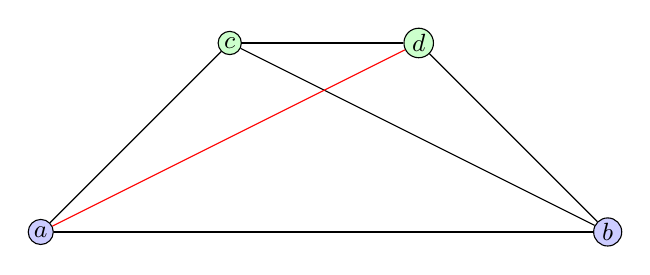
\begin{tikzpicture}[x=1.2cm,y=1.2cm,
    every node/.style={circle,draw,inner sep=1pt,font=\small}]

    % Place K4 vertices
    \node[fill=blue!20]  (a) at (-1,0)   {$a$};
    \node[fill=blue!20]  (b) at (5,0)    {$b$};
    \node[fill=green!20] (c) at (1,2)    {$c$};
    \node[fill=green!20] (d) at (3,2)    {$d$};

    % All edges of K4, with a--d in red
    \foreach \u/\v in {a/b,a/c,b/c,b/d,c/d} {
      \draw (\u) -- (\v);
    }
    \draw[red] (a) -- (d);


    % Track labels

  \end{tikzpicture}
  \caption{A $K_4$ drawn with two “track colors”. No ordering of $a,b,c,d$ can avoid creating a triple $x<y<z$ with $\{x,z\}\in E$ where $y$ shares a track with $x$ or $z$, so at least three tracks are needed.}
  \label{fig:K4-tracks}
\end{figure}

\subsection{A degree bound: $\Delta(G)\le 2k$}

\begin{lemma}[Degree bound for $k$-track nearest-neighbor layouts]
\label{lem:degree-bound}
Let $G = (V,E)$ be a simple undirected graph that is $k$-track nearest-neighbor
representable. That is, there exists a layout $(\tau,p)$ with
\[
  \tau : V \to \{1,\dots,k\}, \qquad
  p : V \to \{1,\dots,|V|\}
\]
such that every edge is legal:
\[
  \forall \{u,v\}\in E,\quad
  v \in N_{\mathrm{legal}}(u)
  \quad\text{(equivalently } u \in N_{\mathrm{legal}}(v)\text{)}.
\]
Then for every vertex $v\in V$ we have
\[
  \deg_G(v) \le 2k.
\]
In particular, the maximum degree $\Delta(G)$ satisfies
\[
  \Delta(G) \le 2k.
\]
\end{lemma}

\begin{proof}
Fix $v\in V$. For each track $t$, let $V_t=\{x:\tau(x)=t\}$ and define
$\operatorname{pred}_t(v),\operatorname{succ}_t(v)$ as before. The legal
neighbor set is
\[
  N_{\mathrm{legal}}(v)
  =
  \{\operatorname{pred}_1(v),\operatorname{succ}_1(v),\dots,
    \operatorname{pred}_k(v),\operatorname{succ}_k(v)\}
  \setminus\{\text{nonexistent}\}.
\]
By nearest-neighbor representability,
\[
  N_G(v) \subseteq N_{\mathrm{legal}}(v),
\]
so
\[
  \deg_G(v) = |N_G(v)| \le |N_{\mathrm{legal}}(v)|.
\]

For each track $t$, at most two vertices can appear in
$N_{\mathrm{legal}}(v)$ from track $t$, namely
$\operatorname{pred}_t(v)$ and $\operatorname{succ}_t(v)$ if they exist.
Define
\[
  S_t(v) :=
    \{\operatorname{pred}_t(v),\operatorname{succ}_t(v)\}
    \setminus\{\text{nonexistent}\},
\]
so $|S_t(v)|\le 2$ and
\[
  N_{\mathrm{legal}}(v)
  = \bigcup_{t=1}^k S_t(v).
\]
Thus
\[
  |N_{\mathrm{legal}}(v)|
  \le \sum_{t=1}^k |S_t(v)|
  \le \sum_{t=1}^k 2
  = 2k.
\]
Hence $\deg_G(v)\le 2k$ for all $v$, and taking the maximum gives
$\Delta(G)\le 2k$.
\end{proof}

\begin{corollary}[Degree-based lower bound on tracks]
\label{cor:tracks-from-degree}
If $G$ is $k$-track nearest-neighbor representable, then
\[
  k \;\ge\; \Bigl\lceil\frac{\Delta(G)}{2}\Bigr\rceil.
\]
\end{corollary}
Figure~\ref{fig:delta5-example} shows a vertex of degree~5, which forces at least three tracks by Corollary~\ref{cor:tracks-from-degree}
\begin{figure}[ht]
  \centering
  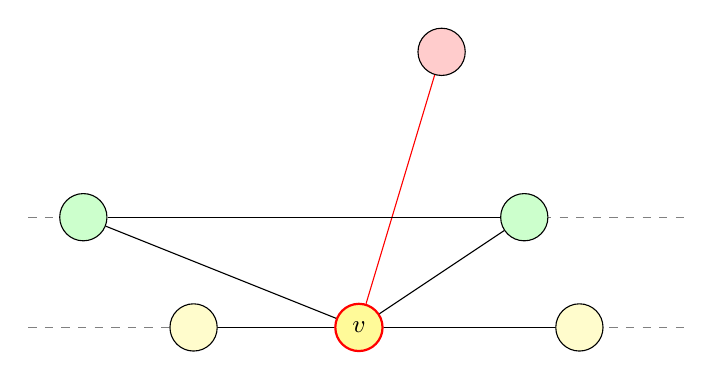
\begin{tikzpicture}[x=1.4cm,y=1.4cm,
    every node/.style={circle,draw,inner sep=1pt,minimum size=6mm,font=\small}]

    % Dashed horizontal lines
    \draw[dashed,gray] (-3,0) -- (3,0);
    \draw[dashed,gray] (-3,1) -- (3,1);

    % Central vertex v
    \node[fill=yellow!40,draw=red,thick] (v) at (0,0) {$v$};

    % Five neighbors around
    \node[fill=yellow!20]  (n1) at (2,0)   {};
    \node[fill=green!20]  (n2) at (1.5,1.0) {};
    \node[fill=red!20]   (n3) at (0.75,2.5)   {};
    \node[fill=green!20] (n4) at (-2.5,1.0) {};
    \node[fill=yellow!20] (n5) at (-1.5,0)  {};

    % Edges: v--n3 in red, others black
    \foreach \w in {n1,n2,n4,n5} {
      \draw (v) -- (\w);
    }
    \draw[red] (v) -- (n3);
    \draw[black] (n2) -- (n4);

  \end{tikzpicture}
  \caption{A vertex of degree $5$: by $\Delta(G)\le 2k$, this implies $k\ge 3$.}
  \label{fig:delta5-example}
\end{figure}

\begin{proof}
Immediate from Lemma~\ref{lem:degree-bound}.
\end{proof}



\begin{figure}[ht]
  \centering
  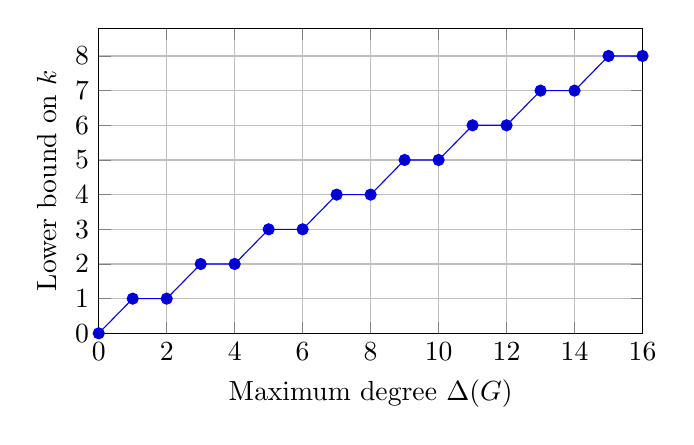
\begin{tikzpicture}
    \begin{axis}[
      width=0.7\textwidth,
      height=0.45\textwidth,
      xlabel={Maximum degree $\Delta(G)$},
      ylabel={Lower bound on $k$},
      ymin=0,
      xmin=0,
      xmax=16,
      xtick={0,2,4,6,8,10,12,14,16},
      ytick={0,1,2,3,4,5,6,7,8},
      grid=both,
    ]
      % Stepwise plot of k ≥ ceil(Δ/2)
      \addplot+[mark=*] coordinates {
        (0,0)
        (1,1)
        (2,1)
        (3,2)
        (4,2)
        (5,3)
        (6,3)
        (7,4)
        (8,4)
        (9,5)
        (10,5)
        (11,6)
        (12,6)
        (13,7)
        (14,7)
        (15,8)
        (16,8)
      };
    \end{axis}
  \end{tikzpicture}
  \caption{Lower bound on the number of tracks:
    $k \ge \lceil \Delta(G)/2\rceil$. In particular, $\Delta(G)\ge 5$
    forces $k\ge 3$.}
\end{figure}


\subsection{Edge bounds for two tracks: at most \texorpdfstring{$2n-3$}{2n-3} edges}

So far we have seen that a $k$-track nearest-neighbor layout forces
$\Delta(G)\le 2k$ (Lemma~\ref{lem:degree-bound}). For $k=2$ we can say much
more: not only is the maximum degree at most $4$, but the \emph{total number
of edges} is at most $2n-3$ for an $n$-vertex graph. This matches the familiar
extremal bound for outerplanar graphs.

We work relative to a fixed $2$-track ordered layout $(\tau,p)$ and its host
graph $H(\tau,p)$.

\begin{definition}[Left-degree]
Given a linear order $v_1,\dots,v_n$ of $V(G)$ induced by $p$, the
\emph{left-degree} of $v_i$ is
\[
  \deg^-(v_i)
  := \bigl|\{\,u\in N_G(v_i) : p(u) < p(v_i)\,\}\bigr|.
\]
Equivalently, $\deg^-(v_i)$ counts neighbors of $v_i$ strictly to the left
of $v_i$ in the global order.
\end{definition}

Every edge $\{u,v\}$ is counted exactly once in the sum of left-degrees, at
its right endpoint.

\begin{lemma}[At most one predecessor per track]
\label{lem:left-degree-two}
Let $G$ be $k$-track nearest-neighbor representable with respect to
$(\tau,p)$, and let $v\in V(G)$. Then for each track $t\in\{1,\dots,k\}$,
$v$ has at most one neighbor on track $t$ to its left. In particular,
\[
  \deg^-(v) \;\le\; k
\]
for every vertex $v$.
\end{lemma}

\begin{proof}
Fix $v$ and a track $t$. By definition, the only candidate left neighbor of
$v$ on track $t$ that is legal in the host graph is $\operatorname{pred}_t(v)$
(if it exists). There cannot be two distinct neighbors $x,y$ on track $t$
with $p(x)<p(y)<p(v)$ and both adjacent to $v$, because only the closest one
to the left can be a legal predecessor on that track.

Thus, on track $t$, there is at most one neighbor of $v$ to the left. Summing
over the $k$ tracks gives $\deg^-(v)\le k$.
\end{proof}

\begin{theorem}[Edge bound for two-track nearest-neighbor layouts]
\label{thm:edge-bound-2tracks}
Let $G$ be a finite simple graph on $n$ vertices that is $2$-track
nearest-neighbor representable. Then
\[
  |E(G)| \;\le\; 2n - 3.
\]
Moreover, for every $n\ge 2$ there exists such a graph with exactly
$2n-3$ edges.
\end{theorem}

\begin{proof}
Let $(\tau,p)$ be a $2$-track layout and let $H=H(\tau,p)$ be its host graph.
Since $G$ is a subgraph of $H$, it suffices to prove $|E(H)|\le 2n-3$.

Write $V=\{v_1,\dots,v_n\}$ in increasing order of $p$, so $p(v_i)=i$. Every
edge of $H$ has a unique right endpoint, so
\[
  |E(H)| = \sum_{i=1}^n \deg_H^-(v_i).
\]

Now:
\begin{itemize}[leftmargin=2em]
  \item For $v_1$, there are no vertices to the left, so $\deg_H^-(v_1)=0$.
  \item For $v_2$, the only vertex to the left is $v_1$, so
        $\deg_H^-(v_2)\le 1$ in any simple graph.
  \item For each $i\ge 3$, Lemma~\ref{lem:left-degree-two} with $k=2$ gives
        $\deg_H^-(v_i)\le 2$.
\end{itemize}
Therefore,
\[
  |E(H)|
  = \sum_{i=1}^n \deg_H^-(v_i)
  \;\le\; 0 + 1 + 2(n-2)
  = 2n - 3.
\]
Since $G$ is a subgraph of $H$, we also have $|E(G)|\le |E(H)|\le 2n-3$.

\medskip
For tightness, fix $n\ge 2$ and construct a $2$-track layout on vertices
$v_1,\dots,v_{n-1},w$ as follows:
\begin{itemize}[leftmargin=2em]
  \item Put $v_1,\dots,v_{n-1}$ on track~1 in the order
        $p(v_i)=i$ and connect all consecutive pairs
        $\{v_i,v_{i+1}\}$, forming a path of length $n-2$.
  \item Put $w$ on track~2 at the far right, $p(w)=n$.
\end{itemize}
On track~1 we have $n-2$ edges. For the cross-track neighbors:
\begin{itemize}[leftmargin=2em]
  \item For each $v_i$, $w$ is the nearest track-2 vertex to the right, so
        $\{v_i,w\}$ is a legal cross-track edge.
  \item There are $n-1$ such vertices $v_i$.
\end{itemize}
Thus $H$ has $(n-2)$ edges along track~1 and $(n-1)$ cross edges to $w$, for
a total of
\[
  (n-2) + (n-1) = 2n - 3
\]
edges. Taking $G=H$ shows that the bound is tight for every $n\ge 2$.
\end{proof}

Figure~\ref{fig:two-track-extremal} shows the extremal construction for
$n=6$, and Figure~\ref{fig:two-track-extremal-growth} shows how each newly
added vertex can contribute at most two new edges when we build such a graph
from left to right in the global order.

\begin{figure}[ht]
  \centering
  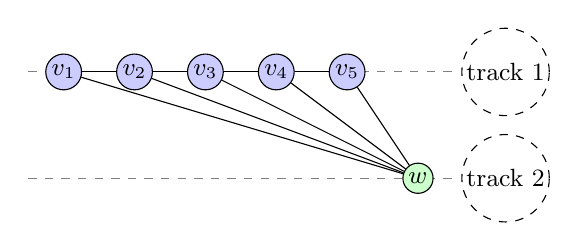
\begin{tikzpicture}[scale=0.9,
    every node/.style={circle,draw,inner sep=1.1pt,font=\small}]
    % Track y-coordinates
    \def\yone{1.5}
    \def\ytwo{0.0}

    % Tracks
    \draw[dashed,gray] (0.5,\yone) -- (6.5,\yone)
      node[right=1mm,black] {$\text{track }1$};
    \draw[dashed,gray] (0.5,\ytwo) -- (6.5,\ytwo)
      node[right=1mm,black] {$\text{track }2$};

    % Vertices on track 1: v1,...,v5
    \foreach \i in {1,...,5} {
      \node[fill=blue!20] (v\i) at (\i,\yone) {$v_{\i}$};
    }

    % Vertex w on track 2 at the far right
    \node[fill=green!20] (w) at (6,\ytwo) {$w$};

    % Path edges on track 1
    \foreach \i/\j in {1/2,2/3,3/4,4/5} {
      \draw (v\i) -- (v\j);
    }

    % Cross edges from w to all v_i
    \foreach \i in {1,...,5} {
      \draw (w) -- (v\i);
    }

  \end{tikzpicture}
  \caption{An extremal $2$-track host graph on $n=6$ vertices:
  a path $v_1-\dots-v_5$ on track~1 and a single vertex $w$ on track~2,
  joined to every $v_i$. This has $(6-2)+(6-1)=9=2n-3$ edges.}
  \label{fig:two-track-extremal}
\end{figure}

\begin{figure}[ht]
  \centering
  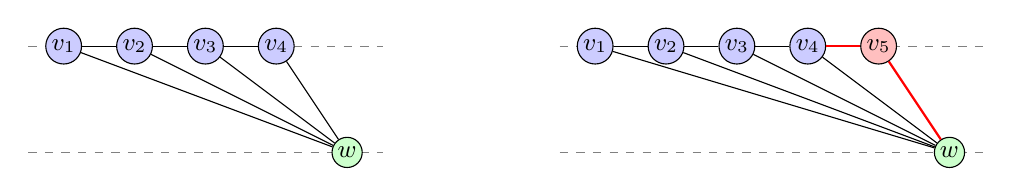
\begin{tikzpicture}[scale=0.9,
    every node/.style={circle,draw,inner sep=1.1pt,font=\small}]

    %==================== Before: n-1 vertices ====================
    \begin{scope}
      \def\yone{1.5}
      \def\ytwo{0.0}

      % Tracks
      \draw[dashed,gray] (0.5,\yone) -- (5.5,\yone);
      \draw[dashed,gray] (0.5,\ytwo) -- (5.5,\ytwo);

      % Vertices on track 1: v1,...,v4
      \foreach \i in {1,...,4} {
        \node[fill=blue!20] (a\i) at (\i,\yone) {$v_{\i}$};
      }

      % Vertex w on track 2
      \node[fill=green!20] (aw) at (5,\ytwo) {$w$};

      % Path edges on track 1
      \foreach \i/\j in {1/2,2/3,3/4} {
        \draw (a\i) -- (a\j);
      }

      % Cross edges from w to all v_i
      \foreach \i in {1,...,4} {
        \draw (aw) -- (a\i);
      }

    \end{scope}

    %==================== After: n vertices ====================
    \begin{scope}[xshift=7.5cm]
      \def\yone{1.5}
      \def\ytwo{0.0}

      % Tracks
      \draw[dashed,gray] (0.5,\yone) -- (6.5,\yone);
      \draw[dashed,gray] (0.5,\ytwo) -- (6.5,\ytwo);

      % Vertices on track 1: v1,...,v5
      \foreach \i in {1,...,4} {
        \node[fill=blue!20] (b\i) at (\i,\yone) {$v_{\i}$};
      }
      % New vertex v5
      \node[fill=red!25] (b5) at (5,\yone) {$v_{5}$};

      % Vertex w on track 2
      \node[fill=green!20] (bw) at (6,\ytwo) {$w$};

      % Old path edges
      \foreach \i/\j in {1/2,2/3,3/4} {
        \draw (b\i) -- (b\j);
      }

      % New path edge and cross edge in red
      \draw[thick,red] (b4) -- (b5);
      \draw[thick,red] (b5) -- (bw);

      % Old cross edges from w to v1,...,v4
      \foreach \i in {1,...,4} {
        \draw (bw) -- (b\i);
      }

    \end{scope}

  \end{tikzpicture}
  \caption{Incremental view of the extremal family. When we append a new
  vertex at the right end of the main track (here $v_5$), we can connect
  it to at most two new neighbors to its left: the previous endpoint of
  the path and the special vertex $w$ on the other track. This contributes
  exactly two new edges, consistent with the bound $|E|\le 2n-3$.}
  \label{fig:two-track-extremal-growth}
\end{figure}


\subsection{Two low-degree vertices at the ends of the order}

The proof of Theorem~\ref{thm:edge-bound-2tracks} naturally singles out the
first and last vertices in the global order. For $k=2$ they \emph{always}
have degree at most~$2$.

\begin{lemma}[Endpoints have degree at most two]
\label{lem:endpoints-degree-two}
Let $G$ be $2$-track nearest-neighbor representable with layout $(\tau,p)$ on
vertices $v_1,\dots,v_n$ in increasing $p$-order. Then
\[
  \deg_G(v_1) \le 2
  \quad\text{and}\quad
  \deg_G(v_n) \le 2.
\]
\end{lemma}

\begin{proof}
By definition,
\[
  N_{\mathrm{legal}}(v)
  =
  \{\operatorname{pred}_1(v),\operatorname{succ}_1(v),
    \operatorname{pred}_2(v),\operatorname{succ}_2(v)\}
  \setminus\{\text{nonexistent}\}.
\]

For $v_1$ there is no vertex to the left on any track, so both
$\operatorname{pred}_1(v_1)$ and $\operatorname{pred}_2(v_1)$ are nonexistent.
The only possible legal neighbors of $v_1$ are its two successors,
$\operatorname{succ}_1(v_1)$ and $\operatorname{succ}_2(v_1)$, one on each
track if they exist. Thus $|N_{\mathrm{legal}}(v_1)|\le 2$, and since
$G$ is a subgraph of the host graph,
$\deg_G(v_1)\le |N_{\mathrm{legal}}(v_1)|\le 2$.

Symmetrically, $v_n$ has no vertices to the right on any track, so both
$\operatorname{succ}_1(v_n)$ and $\operatorname{succ}_2(v_n)$ are nonexistent,
and its only possible legal neighbors are the two predecessors
$\operatorname{pred}_1(v_n)$ and $\operatorname{pred}_2(v_n)$. Again
$|N_{\mathrm{legal}}(v_n)|\le 2$, so $\deg_G(v_n)\le 2$.
\end{proof}

In particular, every connected $2$-track nearest-neighbor representable graph
has at least two vertices of degree at most~$2$, sitting at the left and
right ends of the global order. This is exactly what one needs to start an
inductive ``peeling'' argument: delete $v_1$ or $v_n$, apply the edge bound to
the remaining $(n-1)$-vertex graph, and then add back a vertex of degree at
most~$2$.

\begin{figure}[ht]
  \centering
  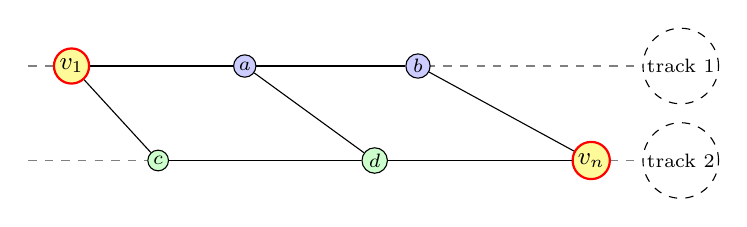
\begin{tikzpicture}[x=1.1cm,y=1.0cm,
    every node/.style={circle,draw,inner sep=1pt,font=\scriptsize}]

    % Tracks
    \draw[dashed,gray] (0.5,1.2) -- (7.5,1.2)
      node[right=1mm,black] {\scriptsize track 1};
    \draw[dashed,gray] (0.5,0.0) -- (7.5,0.0)
      node[right=1mm,black] {\scriptsize track 2};

    % Endpoints
    \node[fill=yellow!40,draw=red,thick,font=\small] (v1) at (1,1.2) {$v_1$};
    \node[fill=yellow!40,draw=red,thick,font=\small] (vn) at (7,0.0) {$v_n$};

    % Middle vertices
    \node[fill=blue!20] (a)  at (3,1.2) {$a$};
    \node[fill=blue!20] (b)  at (5,1.2) {$b$};
    \node[fill=green!20] (c) at (2,0.0) {$c$};
    \node[fill=green!20] (d) at (4.5,0.0) {$d$};

    % Possible neighbors of v1: one on each track
    \draw (v1) -- (a);
    \draw (v1) -- (c);

    % Possible neighbors of vn: one on each track
    \draw (vn) -- (b);
    \draw (vn) -- (d);

    % Some extra edges among middle vertices (just for context)
    \draw (a) -- (b);
    \draw (c) -- (d);
    \draw (a) -- (d);

  \end{tikzpicture}
  \caption{In a $2$-track nearest-neighbor layout, the first vertex $v_1$
  can only see one successor on each track, and the last vertex $v_n$ can
  only see one predecessor on each track. Hence both have degree at most~$2$.}
  \label{fig:endpoints-degree-two}
\end{figure}


% =====================================================
\section{Examples: Cycles and Paths with One Extra Edge}
% =====================================================

We now look at explicit families of graphs and determine their track
numbers, answering more concretely when $k=1$ versus $k=2$ is sufficient.

\subsection{Cycles: $C_n$ needs exactly two tracks}

\begin{theorem}[Track number of a cycle]
\label{thm:cycle}
For every integer $n \ge 3$, the cycle graph $C_n$ is $k$-track nearest-neighbor
representable for $k=2$, but not for $k=1$. In particular,
\[
  \operatorname{tn}(C_n) = 2.
\]
\end{theorem}

\begin{proof}
\emph{Step 1: $C_n$ is not representable with $k=1$.}

Assume, for contradiction, that $C_n$ is $1$-track nearest-neighbor representable.
Then there exists a $1$-track ordered layout $(\tau,p)$ such that every edge of
$C_n$ is legal.

Since $k=1$, every vertex lies on track $1$, and we can write the linear
order as
\[
  v_1, v_2, \dots, v_n, \quad \text{where } p(v_i) = i.
\]
On the single track, the only possible legal edges are between consecutive
vertices:
\[
  E\bigl(H(\tau,p)\bigr) \subseteq \{\{v_i,v_{i+1}\} : 1\le i\le n-1\},
\]
so $H(\tau,p)$ is a forest (in fact a path) and contains no cycle. But
$C_n$ is a cycle, so it cannot be a subgraph of $H(\tau,p)$, contradicting
nearest-neighbor representability.

Thus $C_n$ is not $1$-track representable.

\medskip
\noindent\emph{Step 2: explicit $2$-track layout for $C_n$.}

Label the vertices of $C_n$ as $v_1,\dots,v_n$ with edges
\[
  E(C_n) = \bigl\{\{v_i,v_{i+1}\} : 1\le i \le n-1\bigr\} \cup \{\{v_n,v_1\}\}.
\]

\smallskip
\noindent\emph{Global order.}
Set $p(v_i)=i$ for all $i$.

\smallskip
\noindent\emph{Track assignment.}
Use two tracks $\{1,2\}$ and define
\[
  \tau(v_1) = \tau(v_n) = 1, \qquad
  \tau(v_i) = 2 \quad \text{for } 2 \le i \le n-1.
\]
Thus track $1$ has vertices $\{v_1,v_n\}$ and track $2$ has
$\{v_2,\dots,v_{n-1}\}$.

We now check that each edge of $C_n$ is legal.

\smallskip
\noindent\emph{Interior edges on track 2.}
For $2\le i\le n-2$, both $v_i$ and $v_{i+1}$ lie on track $2$ and are
consecutive there, so
\[
  \operatorname{succ}_2(v_i) = v_{i+1},\quad
  \operatorname{pred}_2(v_{i+1}) = v_i.
\]
Hence each $\{v_i,v_{i+1}\}$ with $2\le i\le n-2$ is legal.

\smallskip
\noindent\emph{Edges $\{v_1,v_2\}$ and $\{v_{n-1},v_n\}$.}
These involve one vertex on track $1$ and one on track $2$.
Checking the nearest opposite-track neighbors shows:
\begin{itemize}[leftmargin=2em]
  \item $v_2$ is the closest track-$2$ vertex to the right of $v_1$
        and $v_1$ is the closest track-$1$ vertex to the left of $v_2$,
        so $\{v_1,v_2\}$ is legal.
  \item $v_n$ is the closest track-$1$ vertex to the right of $v_{n-1}$
        and $v_{n-1}$ is the closest track-$2$ vertex to the left of $v_n$,
        so $\{v_{n-1},v_n\}$ is legal.
\end{itemize}

\smallskip
\noindent\emph{Edge $\{v_n,v_1\}$.}
Both endpoints lie on track $1$ and are the only vertices there, so
\[
  \operatorname{succ}_1(v_1) = v_n,\quad
  \operatorname{pred}_1(v_n) = v_1,
\]
and $\{v_n,v_1\}$ is legal.

\smallskip
Thus $(\tau,p)$ is a $2$-track layout in which all edges of $C_n$ are legal,
so $C_n$ is $2$-track nearest-neighbor representable.

Combined with the non-representability for $k=1$, we obtain
$\operatorname{tn}(C_n)=2$.
\end{proof}

\begin{figure}[h]
  \centering
  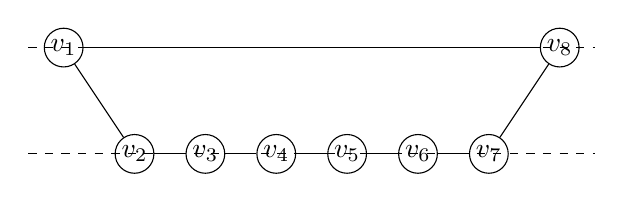
\begin{tikzpicture}[scale=0.9, every node/.style={circle,draw,inner sep=1.1pt}]
    % Track y-coordinates
    \def\yone{1.5}
    \def\ytwo{0}

    % Vertices v1,...,v8 on x=1,...,8
    \foreach \i in {1,...,8} {
      \pgfmathsetmacro{\x}{\i}
      % Track assignment: v1,v8 on track 1; others on track 2
      \ifnum\i=1
        \node (v\i) at (\x,\yone) {$v_{\i}$};
      \else\ifnum\i=8
        \node (v\i) at (\x,\yone) {$v_{\i}$};
      \else
        \node (v\i) at (\x,\ytwo) {$v_{\i}$};
      \fi\fi
    }

    % Draw tracks as dashed lines
    \draw[dashed] (0.5,\yone) -- (8.5,\yone);
    \draw[dashed] (0.5,\ytwo) -- (8.5,\ytwo);

    % Cycle edges: (v1-v2-...-v8-v1)
    \foreach \i/\j in {1/2,2/3,3/4,4/5,5/6,6/7,7/8,8/1} {
      \draw (v\i) -- (v\j);
    }
  \end{tikzpicture}
  \caption{A $2$-track layout of $C_8$ with $v_1,v_8$ on track~1 and $v_2,\dots,v_7$ on track~2.}
\end{figure}

\subsection{A path plus one extra edge}

We next show that a path with a single additional edge is always
$2$-track representable. This is a simple example of a graph that is
\emph{no longer} a linear forest but still only needs $k=2$ tracks.

\begin{theorem}[Paths with one extra edge]
\label{thm:path-plus-edge}
Let $G$ be a connected simple undirected graph obtained as follows:
\begin{itemize}[leftmargin=2em]
  \item $V = \{v_1,\dots,v_n\}$ for some $n \ge 2$,
  \item $E$ contains all path edges $\{v_i,v_{i+1}\}$ for $i = 1,\dots,n-1$,
  \item and in addition a single extra edge $e^\star = \{v_a,v_b\}$ with $1 \le a < b \le n$.
\end{itemize}
Then $G$ is $2$-track nearest-neighbor representable.
\end{theorem}
Figure~\ref{fig:path-plus-edge-interior} illustrates the construction in the case of an extra edge $\{v_3,v_7\}$. The same idea works when one or both endpoints of the extra edge are at the ends of the path. Since a $1$-track nearest-neighbor representable graph is a linear forest
(Remark~\ref{rem:what-k1-means}) and our graphs contain a cycle, they cannot
be $1$-track representable. Combined with the construction above, this shows
that their nearest-neighbor track number is exactly $2$.

\begin{figure}[ht]
  \centering
  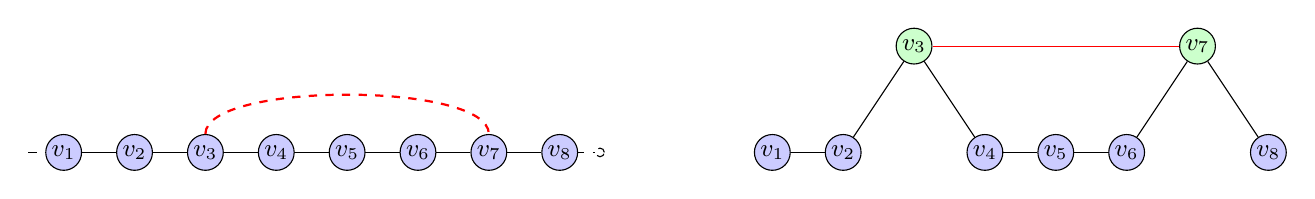
\begin{tikzpicture}[scale=0.9,
    every node/.style={circle,draw,inner sep=1.1pt,font=\small}]

    %==================== Before: 1-track layout ====================
    \begin{scope}
      % Single track
      \def\ybefore{0}
      \draw[dashed] (0.5,\ybefore) -- (8.5,\ybefore)
        node[right] {};

      % Vertices v1,...,v8 on the single track
      \foreach \i in {1,...,8} {
        \node[fill=blue!20] (u\i) at (\i,\ybefore) {$v_{\i}$};
      }

      % Path edges (all legal in 1-track layout)
      \foreach \i/\j in {1/2,2/3,3/4,4/5,5/6,6/7,7/8} {
        \draw (u\i) -- (u\j);
      }

      % Extra edge {v3,v7}: not a nearest-neighbor edge here
      \draw[thick,red,dashed] (u3) .. controls +(0,1.0) and +(0,1.0) .. (u7);


    \end{scope}

    %==================== After: 2-track layout ====================
    \begin{scope}[xshift=10cm]
      % Track y-coordinates
      \def\yone{0}
      \def\ytwo{1.5}

      % Vertices v1,...,v8
      \foreach \i in {1,...,8} {
        \ifnum\i=3
          \node[fill=green!20] (v\i) at (\i,\ytwo) {$v_{\i}$}; % a = 3 elevated
        \else\ifnum\i=7
          \node[fill=green!20] (v\i) at (\i,\ytwo) {$v_{\i}$}; % b = 7 elevated
        \else
          \node[fill=blue!20]  (v\i) at (\i,\yone) {$v_{\i}$};
        \fi\fi
      }

      % Path edges (still all legal)
      \foreach \i/\j in {1/2,2/3,3/4,4/5,5/6,6/7,7/8} {
        \draw (v\i) -- (v\j);
      }

      \draw[red] (v3) -- (v7);
      % Caption under the right subgraph
    \end{scope}

  \end{tikzpicture}
  \caption{A path $v_1-\cdots-v_8$ with an extra edge $\{v_3,v_7\}$. 
  Left: the natural $1$-track layout of the path; the extra edge (red, dashed) skips several vertices and is not a nearest-neighbor edge. 
  Right: by moving $v_3$ and $v_7$ to track~2, we obtain a $2$-track nearest-neighbor layout in which the extra edge (solid red) becomes legal while all path edges remain legal.}
  \label{fig:path-plus-edge-interior}
\end{figure}


\begin{proof}
We keep the natural order $p(v_i)=i$ and modify only the track assignment.

\smallskip
\noindent\emph{Step 1: start with the path.}
For the bare path $P_n$ with edges $\{v_i,v_{i+1}\}$, the layout
\[
  \tau^{(1)}(v_i) = 1\quad\text{for all }i,
  \qquad p(v_i)=i,
\]
is a $1$-track nearest-neighbor layout: each $\{v_i,v_{i+1}\}$ connects
consecutive vertices on track $1$.

\smallskip
\noindent\emph{Step 2: move the extra-edge endpoints to track 2.}
Now add the extra edge $e^\star=\{v_a,v_b\}$ with $a<b$, keep the same
global order $p$, and define a new track assignment $\tau$ by
\[
  \tau(v_i) =
  \begin{cases}
    2, & \text{if } i \in \{a,b\},\\[2pt]
    1, & \text{otherwise}.
  \end{cases}
\]
Thus only $v_a$ and $v_b$ are on track $2$; every other vertex is on track $1$.

We check that every edge of $G$ is legal under $(\tau,p)$.

\smallskip
\noindent\emph{Step 3: path edges not incident with $v_a$ or $v_b$.}
If $i\notin\{a-1,a,b-1,b\}$, then
$\{v_i,v_{i+1}\}$ is not incident with $v_a$ or $v_b$ and both endpoints
lie on track $1$. They are consecutive in the global order, and no other
track-$1$ vertex lies between them; hence
\[
  \operatorname{succ}_1(v_i)=v_{i+1},\quad
  \operatorname{pred}_1(v_{i+1})=v_i,
\]
and $\{v_i,v_{i+1}\}$ is legal.

\smallskip
\noindent\emph{Step 4: path edges incident with $v_a$ or $v_b$.}
Consider the edges $\{v_{a-1},v_a\}$ and $\{v_a,v_{a+1}\}$ (when these
indices exist). The neighbor of $v_a$ immediately to the left on track $1$
is $v_{a-1}$ and immediately to the right is $v_{a+1}$, so
\[
  \operatorname{pred}_1(v_a) = v_{a-1}\text{ (if $a>1$)},\quad
  \operatorname{succ}_1(v_a) = v_{a+1}\text{ (if $a<n$)}.
\]
Thus the edges $\{v_{a-1},v_a\}$ and $\{v_a,v_{a+1}\}$ are legal.

The same argument applies to $v_b$: the nearest track-$1$ vertices to the left
and right are $v_{b-1}$ and $v_{b+1}$ (when they exist), making
$\{v_{b-1},v_b\}$ and $\{v_b,v_{b+1}\}$ legal.

\smallskip
\noindent\emph{Step 5: the extra edge $\{v_a,v_b\}$.}
On track $2$, $v_a$ and $v_b$ are the only vertices and $a<b$. Thus
\[
  \operatorname{succ}_2(v_a) = v_b, \qquad
  \operatorname{pred}_2(v_b) = v_a,
\]
so $v_b\in N_{\mathrm{legal}}(v_a)$ and $v_a\in N_{\mathrm{legal}}(v_b)$.
Hence the extra edge is legal.

\smallskip
Altogether, every edge of $G$ is legal, so $G$ is $2$-track
nearest-neighbor representable.
\end{proof}

% =====================================================
\section{Planarity for $k\le 2$}
% =====================================================

Finally, we show that $k\le 2$ imposes strong structural limitations:
every such graph is planar.

\begin{theorem}[Planarity for $k\le 2$]
\label{thm:planarity-k-le-2}
Let $G$ be a simple undirected graph that is $(k)$-track nearest-neighbor
representable with $k\le 2$. Then $G$ is planar.
\end{theorem}

\begin{proof}
We treat $k=1$ and $k=2$ separately.

\medskip
\noindent\emph{Case $k=1$.}
When there is only one track, each vertex has at most one predecessor
and one successor, and every legal edge joins consecutive vertices in
the single track order. Thus every connected component of $G$ is a path
(or an isolated vertex). Such a graph is a disjoint union of paths and
isolated vertices, hence planar.

\medskip
\noindent\emph{Case $k=2$: reduction to host graphs.}
Fix a $2$-track layout $(\tau,p)$ on $V$ and let $H(\tau,p)$ be the host
graph containing all legal edges. Since $G$ is a subgraph of $H(\tau,p)$,
it suffices to show that $H(\tau,p)$ is planar.

Place the vertices along a horizontal line in the global order
$v_1,\dots,v_n$ with $p(v_i)=i$, and write $\tau(v_i)\in\{1,2\}$.
We partition the edges of $H(\tau,p)$ into four classes:

\begin{itemize}[leftmargin=2em]
  \item $E^{(1)}$: edges between consecutive vertices on track $1$,
  \item $E^{(2)}$: edges between consecutive vertices on track $2$,
  \item $E_R$: cross-track edges where each vertex is the nearest opposite-track
               neighbor to the right,
  \item $E_L$: cross-track edges where each vertex is the nearest opposite-track
               neighbor to the left.
\end{itemize}

Figure~\ref{fig:planar-2tracks} schematically illustrates the planar drawing used in the proof.
\begin{figure}[ht]
  \centering
  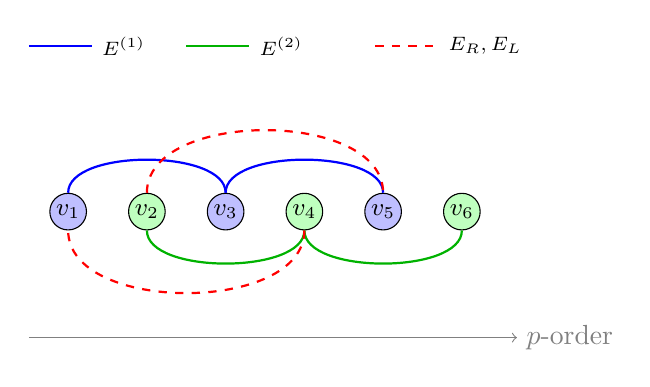
\begin{tikzpicture}[x=1.0cm,y=1cm]

    % Vertices on the x-axis, colored by track
    \foreach \i/\x/\col in {1/1/blue!25,2/2/green!25,3/3/blue!25,4/4/green!25,5/5/blue!25,6/6/green!25} {%
      \node[circle,draw,fill=\col,inner sep=1.2pt,font=\small] (v\i) at (\x,0) {$v_{\i}$};
    }

    % p-order arrow
    \draw[->,gray] (0.5,-1.6) -- (6.7,-1.6) node[right] {$p$-order};

    % Edges on track 1 (E^{(1)}) in upper half-plane
    \draw[thick,blue] (v1) .. controls +(0,0.8) and +(0,0.8) .. (v3);
    \draw[thick,blue] (v3) .. controls +(0,0.8) and +(0,0.8) .. (v5);

    % Edges on track 2 (E^{(2)}) in lower half-plane
    \draw[thick,green!70!black] (v2) .. controls +(0,-0.8) and +(0,-0.8) .. (v4);
    \draw[thick,green!70!black] (v4) .. controls +(0,-0.8) and +(0,-0.8) .. (v6);

    % Cross edges to the right (E_R) in upper half-plane
    \draw[thick,red,dashed] (v2) .. controls +(0,1.3) and +(0,1.3) .. (v5);

    % Cross edges to the left (E_L) in lower half-plane
    \draw[thick,red,dashed] (v4) .. controls +(0,-1.3) and +(0,-1.3) .. (v1);

    % Legend
    \begin{scope}[shift={(0.5,2.1)},font=\scriptsize]
      \draw[blue,thick] (0,0) -- (0.8,0) node[right,black] {$E^{(1)}$};
      \draw[green!70!black,thick] (2.0,0) -- (2.8,0) node[right,black] {$E^{(2)}$};
      \draw[red,thick,dashed] (4.4,0) -- (5.2,0) node[right,black] {$E_R, E_L$};
    \end{scope}

  \end{tikzpicture}
  \caption{A schematic planar embedding for a $2$-track host graph: edges on track~1 and right-going cross edges are drawn above the line, while edges on track~2 and left-going cross edges are drawn below.}
  \label{fig:planar-2tracks}
\end{figure}

We draw:
\begin{itemize}[leftmargin=2em]
  \item all vertices $v_1,\dots,v_n$ on the $x$-axis at $(i,0)$,
  \item all edges in $E^{(1)}\cup E_R$ as $x$-monotone arcs in the upper
        half-plane,
  \item all edges in $E^{(2)}\cup E_L$ as $x$-monotone arcs in the lower
        half-plane.
\end{itemize}

It is a standard interval-order argument (we omit the routine details) that:

\begin{itemize}[leftmargin=2em]
  \item edges in $E^{(1)}$ form a non-crossing family in the upper half-plane,
  \item edges in $E_R$ form a non-crossing family in the upper half-plane,
  \item no edge in $E^{(1)}$ crosses any edge in $E_R$ in the upper half-plane,
  \item by symmetry, the same holds for $E^{(2)}$ and $E_L$ in the lower half-plane.
\end{itemize}

Since upper and lower half-plane edges only meet along the horizontal
line at their endpoints, this gives a planar embedding of $H(\tau,p)$.
Thus $H(\tau,p)$ is planar, and any subgraph $G$ of it is planar as well.
\end{proof}

This planarity constraint, together with the degree and edge bounds proved
earlier, will be exploited in Section~\ref{sec:recognition} to design a
recognition algorithm for $2$-track nearest-neighbor layouts.


% =====================================================
\section{Complexity: Recognizing 2-Track Nearest-Neighbor Layouts}
% =====================================================


\subsection{The decision problem \textsc{2TNN-Layout}}

We fix $k=2$ throughout this section. Recall that a $2$-track
nearest-neighbor layout of a graph $G=(V,E)$ consists of:
\begin{itemize}[leftmargin=2em]
  \item a track assignment $\tau:V\to\{1,2\}$,
  \item and a bijection $p:V\to\{1,\dots,|V|\}$,
\end{itemize}
such that every edge $\{u,v\}\in E$ is legal in the sense of
Section~1: each endpoint is either the predecessor or successor of the other
on some track (its own or the opposite track).

\begin{definition}[\textsc{2TNN-Layout}]
\label{def:2tnn-layout-problem}
The decision problem \textsc{2TNN-Layout} is:

\medskip\noindent
\emph{Input:} A finite simple undirected graph $G=(V,E)$.

\smallskip\noindent
\emph{Question:} Does there exist a $2$-track ordered layout $(\tau,p)$ of $G$
such that $G$ is $2$-track nearest-neighbor representable with respect to
$(\tau,p)$, i.e.
\[
  \forall v\in V,\quad N_G(v) \subseteq N_{\mathrm{legal}}(v)?
\]
Equivalently, is $\operatorname{tn}(G)\le 2$ in the nearest-neighbor sense?
\end{definition}

\subsection{Membership in NP}

\begin{proposition}[\textsc{2TNN-Layout} is in NP]
\label{prop:2tnn-in-NP}
The problem \textsc{2TNN-Layout} belongs to the complexity class NP.
\end{proposition}

\begin{proof}
A certificate consists of a pair $(\tau,p)$ with $\tau:V\to\{1,2\}$ and a
bijection $p:V\to\{1,\dots,n\}$. From $(\tau,p)$ we can compute all
predecessors and successors along each track in linear time and thus the
legal neighbor sets $N_{\mathrm{legal}}(v)$.
We then verify in $O(|E|)$ time that every edge of $G$ is legal at both
endpoints. Hence \textsc{2TNN-Layout} is in NP.
\end{proof}




% =====================================================
\section{A Recognition Algorithm for Two-Track Layouts}
% =====================================================
\label{sec:recognition}

\begin{quote}
	extbf{Hybrid Algorithm: Two-Track Graph Recognizer}

\emph{Objective:} Efficiently determine if a graph $G$ can be represented with $k \le 2$ tracks.

\emph{Complexity:} $O(N)$ for almost all cases (including all trees). Exponential only in the size of the most complex individual cycle.

	extbf{Phase 1: Global Viability Filters (Necessary Bounds)}
\begin{itemize}
  \item \textbf{Density Filter:} If $|E| > 2|V| - 3$, return \emph{FALSE} (too dense). Cost: $O(1)$.
  \item \textbf{Planarity Filter:} If $G$ is not planar (e.g., contains $K_{3,3}$), return \emph{FALSE}. Cost: $O(N)$.
  \item \textbf{Degree Filter:} If $\Delta(G) \ge 5$, return \emph{FALSE}. Cost: $O(N)$.
\end{itemize}

	extbf{Phase 2: Kernelization (Leaf Peeling)}
\begin{itemize}
  \item Recursively remove all degree-1 vertices (leaves), updating neighbor degrees.
  \item If the original graph was a tree or forest, this phase reduces it to the empty graph. If no nodes remain, return \emph{TRUE}.
  \item The remaining graph is the \emph{core} ($G_{core}$), containing only cycles and closed structures.
\end{itemize}

	extbf{Phase 3: Topological Decomposition (Divide and Conquer)}
\begin{itemize}
  \item Use DFS to find articulation points in the core.
  \item Decompose the core into a list of biconnected components (blocks) $B_1, B_2, \dots$.
  \item Justification: The problem is local; if any block fails, the whole graph fails.
\end{itemize}

	extbf{Phase 4: Exact Solver (Local Validation)}
\begin{itemize}
  \item For each block $B_i$, run a slot-based backtracking solver with $k=2$.
  \item If any block returns \emph{FALSE}, return \emph{FALSE} for the whole graph.
  \item If all blocks succeed, return \emph{TRUE}.
\end{itemize}
\end{quote}

% -----------------------------------------------------
\section{Leyes Fundamentales sobre Tracks y Coloración}

\subsection{Ley de los puntos de articulación y coloración óptima}
\begin{theorem}[Coloring and Articulation Points]
Let $G$ be a connected graph and $v$ an articulation point of $G$. If removing $v$ separates $G$ into components $C_1, C_2, \ldots, C_k$, then:
\begin{itemize}
  \item The chromatic number of $G$ equals the maximum of the chromatic numbers of the induced subgraphs $C_i \cup \{v\}$, for $i = 1, \ldots, k$.
  \item An optimal $k$-coloring of $G$ can be obtained by coloring $v$ and then, for each component $C_i$, coloring $C_i$ separately, ensuring that the neighbors of $v$ in $C_i$ receive a color different from $v$.
\end{itemize}
In summary: The optimal coloring of a graph with an articulation point can be constructed by combining the optimal colorings of the parts separated by that point, respecting the color of the articulation point.
\end{theorem}

\subsection{Ley para bosques y árboles (track number)}
\begin{theorem}[Track Number of Forests and Trees]
A graph $G$ is a forest (i.e., acyclic) if and only if its nearest-neighbor track number is $1$. In particular, every tree admits a $1$-track nearest-neighbor layout.
\end{theorem}
\begin{proof}
A $1$-track layout only allows paths and isolated vertices (a linear forest). Any cycle would require at least two tracks. Thus, $G$ is a forest if and only if it is $1$-track representable.
\end{proof}

\subsection{Ley para el número de tracks en función del grado máximo}
\begin{theorem}[Track Number and Maximum Degree in Forests]
If $G$ is a forest with maximum degree $\Delta$, then its nearest-neighbor track number $k$ satisfies $k = \lceil \Delta/2 \rceil$.
\end{theorem}
\begin{proof}
In a $1$-track layout, each vertex can have at most two neighbors (left and right). For higher degrees, the minimum number of tracks needed is $\lceil \Delta/2 \rceil$ to avoid conflicts.
\end{proof}

\subsection{Leyes algorítmicas para reconocimiento de dos tracks}

% -----------------------------------------------------
\subsection{Additional Algorithmic Laws for Two-Track Recognition}
% -----------------------------------------------------
\begin{theorem}[Memoization of Isomorphic Blocks]
During the decomposition into biconnected blocks, if two blocks are isomorphic (structurally identical), the result of the exact solver for one can be reused for the other.
\end{theorem}
\begin{proof}
Isomorphic blocks have the same constraints and possible layouts. Thus, solving one instance provides a solution for all isomorphic copies, reducing redundant computation and improving efficiency.
\end{proof}

\begin{theorem}[Parallelization of Block Solvers]
The exact validation of each biconnected block is independent of the others. Therefore, the solvers can be executed in parallel for each block.
\end{theorem}
\begin{proof}
Since blocks are separated by articulation points, their layouts do not interfere. Running solvers in parallel leverages multi-core systems, reducing total runtime without affecting correctness.
\end{proof}

\begin{theorem}[Advanced Core Reduction]
If the core contains twin vertices (vertices with identical neighbor sets) or contractible paths, these can be merged or removed without affecting the existence of a two-track nearest-neighbor layout.
\end{theorem}
\begin{proof}
Merging twins or contracting paths preserves the essential connectivity and constraints of the core. These reductions simplify the problem, decrease the exponential search space, and maintain the validity of the recognition algorithm.
\end{proof}


% -----------------------------------------------------
\subsection{Immediate decisions from size and density}
% -----------------------------------------------------

Fix a connected component $H$.

\paragraph{Cut 0: tiny graphs.}
If $n_H \le 3$ then $H$ has at most three edges and no $K_4$, and one easily
writes down a $2$-track nearest-neighbor layout by hand.  We therefore treat
\[
  n_H \le 3 \quad\Longrightarrow\quad \operatorname{tn}(H) \le 2
\]
as an \emph{automatic YES}.  This is checked in $O(1)$ per component.

\paragraph{Cut 1: edge-density upper bound.}
By Theorem~\ref{thm:edge-bound-2tracks}, every $2$-track nearest-neighbor
host graph on $n_H$ vertices has at most $2n_H-3$ edges. Hence any component
with $m_H > 2n_H-3$ cannot have $\operatorname{tn}(H)\le 2$.

% -----------------------------------------------------
\subsection{Linear-time structural filters}
% -----------------------------------------------------

Once $n_H \ge 4$ and $m_H \le 2n_H-3$, we apply three more structural cuts,
each justified by earlier results.

\paragraph{Cut 2: maximum degree.}
By Lemma~\ref{lem:degree-bound}, a $k$-track nearest-neighbor layout satisfies
$\Delta(H)\le 2k$.  For $k\le 2$ this gives
\[
  \Delta(H) \le 4.
\]
Thus if we ever see $\Delta(H)\ge 5$ we can immediately conclude
$\operatorname{tn}(H)\ge 3$ and return \emph{NO}.  Computing all degrees takes
$O(n_H + m_H)$ time.

\paragraph{Cut 3: $K_4$-subgraph.}
Theorem~\ref{thm:K4-needs-3} shows that a $4$-clique forces at least three
tracks.  So if $H$ contains a $K_4$ we must reject:
\[
  K_4 \subseteq H \quad\Longrightarrow\quad \operatorname{tn}(H) \ge 3.
\]
Given $\Delta(H)\le 4$ from Cut~2, $K_4$ can be detected in
$O(n_H \Delta(H)^2) = O(n_H)$ time by intersecting neighbor sets.

\paragraph{Cut 4: planarity.}
By Theorem~\ref{thm:planarity-k-le-2}, any graph with $\operatorname{tn}(H)\le 2$
must be planar.  We therefore run a linear-time planarity test (for example
Hopcroft--Tarjan) and reject if $H$ is nonplanar:
\[
  H \text{ nonplanar } \quad\Longrightarrow\quad \operatorname{tn}(H)\ge 3.
\]
This is $O(n_H + m_H)$.

After Cuts 1--4 all remaining components satisfy simultaneously
\[
  n_H \ge 4,\quad
  m_H \le 2n_H - 3,\quad
  \Delta(H) \le 4,\quad
  H \text{ planar},\quad
  K_4 \not\subseteq H.
\]

% -----------------------------------------------------
\subsection{Cheap YES cases}
% -----------------------------------------------------

Before we resort to any backtracking, we also exploit explicit constructions
from Section~5.

\paragraph{Cut 5: linear forests.}
If every component of $H$ is a path or an isolated vertex (a linear forest),
then $\operatorname{tn}(H)=1$ by the discussion in Section~1, and we answer
\emph{YES}.  In the connected case this is simply the test
\[
  \Delta(H) \le 2\quad \text{and $H$ acyclic}.
\]
Acyclicity and degrees can both be checked in $O(n_H+m_H)$.

\paragraph{Cut 6: one cycle with maximum degree $2$.}
Section~5 proves that
\begin{itemize}[leftmargin=2em]
  \item every cycle $C_n$ has $\operatorname{tn}(C_n)=2$
        (Theorem~\ref{thm:cycle}), and
  \item any graph obtained from a path by adding one extra edge is also
        $2$-track nearest-neighbor representable
        (Theorem~\ref{thm:path-plus-edge}).
\end{itemize}
These are precisely the connected graphs with
\[
  m_H = n_H,\quad \Delta(H) \le 2,
\]
i.e.\ graphs with as many edges as vertices and maximum degree at most two.

Thus connected components with
\[
  m_H = n_H \quad\text{and}\quad \Delta(H)\le 2
\]
are \emph{automatic YES} and never reach the expensive search layer.  Again,
this test is $O(n_H+m_H)$.

(One can extend this family further if desired, using more structure theorems,
but the above already covers the most common sparse unicyclic cases.)

% -----------------------------------------------------
\subsection{Reducing to a bounded-degree planar core}
% -----------------------------------------------------
\label{subsec:two-track-core}
After Cuts 0--6, only ``genuinely complicated'' components remain: planar,
$K_4$-free graphs with $3 \le \delta(H)\le \Delta(H)\le 4$ and
$m_H\le 2n_H-3$ that are neither linear forests nor simple cycles nor
paths-with-one-extra-edge.

At this point we shrink $H$ to a smaller \emph{core} $H^\star$ by deleting
inessential leaves and degree-$2$ path vertices, in the spirit of standard
kernelization.

\begin{itemize}[leftmargin=2em]
  \item While $H$ has a leaf $v$ (degree $1$), delete $v$ and its incident edge.
        By the usual ``attach-the-leaf-back'' argument, this does not change
        whether a $2$-track nearest-neighbor layout exists.
  \item While $H$ has a degree-$2$ vertex $v$ whose neighbors $x,y$ are not
        adjacent, contract the path $x-v-y$ to a single edge $xy$.  This
        preserves the existence of a layout as well: in any layout of the
        contracted graph, $v$ can be reinserted along the track between $x$
        and $y$.
\end{itemize}

We call the result $H^\star$ the \emph{two-track core} of $H$.  It is planar,
$K_4$-free, has $3 \le \delta(H^\star) \le \Delta(H^\star) \le 4$, and can be
computed in $O(n_H+m_H)$.

If $H^\star$ is empty, or a single vertex, or a single cycle, we already know
how to layout $H$ from previous cuts; otherwise, $H^\star$ is the instance on
which we run the exponential search.

% -----------------------------------------------------
\subsection{The backtracking layer}
% -----------------------------------------------------

On $H^\star$ we now run a backtracking algorithm that is exact but exponential
in the size of $H^\star$.  The key observation is that for $k=2$ every vertex
$v$ can use at most four legal nearest-neighbor positions:

\[
  \{\text{pred on track 1},\ \text{succ on track 1},\
    \text{pred on track 2},\ \text{succ on track 2}\}.
\]

We encode these as four abstract \emph{slots}
\[
  \mathsf{1L},\ \mathsf{1R},\ \mathsf{2L},\ \mathsf{2R},
\]
and we search over assignments of incident edges to slots, subject to:

\begin{itemize}[leftmargin=2em]
  \item at each vertex, at most one edge uses each slot (degree bound),
  \item at each edge $\{u,v\}$, the pair of slots chosen at $u$ and $v$ must
        be one of the eight compatible pairs coming from an actual
        predecessor/successor relation (same-track or cross-track), and
  \item the induced ``to-the-left-of'' constraints on vertices must stay
        acyclic, so that they can be realized by a global order~$p$.
\end{itemize}

We maintain partial slot assignments and their implications as a standard
finite-domain CSP, and we branch on a vertex with fewest available slots.
Since $\deg(v)\le 4$ and there are four slots, the local branching factor is
at most $4! = 24$, and usually much smaller once constraints are propagated.

A complete, consistent assignment of slots yields a $2$-track nearest-neighbor
layout of $H^\star$ (and hence of $H$), while failure on all branches proves
that no such layout exists.  The correctness argument is routine and follows
the same pattern as other layout/ordering CSPs; the details are omitted here
for brevity.

In the worst case this backtracking layer runs in time
\[
  O\bigl(c^{n^\star}\bigr),
\]
for some constant $c<24$ and $n^\star = |V(H^\star)|$, multiplied by a
polynomial factor for constraint propagation.  This exponential behavior is
expected: already the standard track-number recognition problem for fixed
$k=2$ is NP-complete
(see Dujmovi\'c et al.~\cite{dujmovic-track-layouts,dujmovic-layered-track}).

% -----------------------------------------------------
\subsection{Final algorithm and global complexity}
% -----------------------------------------------------

We can now summarize the whole procedure.

\begin{quote}
\textbf{Algorithm \textsc{TwoTrackNN}$(G)$}

\emph{Input:} finite simple graph $G=(V,E)$. \\
\emph{Output:} $1$ if $G$ has a nearest-neighbor layout with at most two
tracks, $0$ otherwise.

\begin{enumerate}[leftmargin=2em]
  \item Compute connected components $G_1,\dots,G_r$ of $G$ \hfill
        (time $O(|V|+|E|)$).
  \item For each component $G_i$:
    \begin{enumerate}[label=(\alph*),leftmargin=1.5em]
      \item Let $n_i = |V(G_i)|$, $m_i = |E(G_i)|$.
            If $n_i \le 3$, mark $G_i$ as \emph{YES} and continue.
      \item If $m_i > 2n_i - 3$, return $0$ (Cut~1).
      \item Compute degrees.  If $\Delta(G_i) \ge 5$, return $0$ (Cut~2).
      \item Test for a $K_4$; if found, return $0$ (Cut~3).
      \item Run a linear-time planarity test; if $G_i$ is nonplanar,
            return $0$ (Cut~4).
      \item If $G_i$ is a linear forest, or a cycle, or a path plus one
            extra edge (Cuts 5 and 6), mark it as \emph{YES} and continue.
      \item Otherwise compute its core $G_i^\star$ by repeatedly deleting
            leaves and suppressing degree-$2$ path vertices (Section~\ref{subsec:two-track-core}).
      \item Run the slot-based backtracking search on $G_i^\star$.
            If it fails, return $0$; if it succeeds, mark $G_i$ as
            \emph{YES}.
    \end{enumerate}
  \item If all components are marked \emph{YES}, return $1$.
\end{enumerate}
\end{quote}

Steps (1)--(2f) and the core reduction (2g) together take
\[
  O(|V| + |E|)
\]
time.


% =====================================================
\begin{thebibliography}{9}


\bibitem{dujmovic-layered-track}
V.~Dujmovi\'c and D.~R.~Wood.
Track layouts, layered path decompositions, and leveled planarity.
\emph{Journal of Graph Theory}, to appear.
Preprint available as arXiv:1506.09145.

\bibitem{hopcroft-tarjan}
J.~Hopcroft and R.~Tarjan.
Efficient planarity testing.
\emph{Journal of the ACM} 21(4):549--568, 1974.

\bibitem{queue-number-survey}
D.~Eppstein.
Queue number.
Available at \url{https://en.wikipedia.org/wiki/Queue_number}.

% =====================================================
\end{thebibliography}
% =====================================================
\appendix
% =====================================================
\section{Failed BFS-Based Cut Attempts}
% =====================================================
\label{app:failed-bfs-cuts}

During the design of the recognition algorithm in
Section~\ref{sec:recognition} it is tempting to look for extra ``cheap''
necessary conditions coming from the behavior of breadth-first search (BFS).
In this appendix we record two such ideas that turned out to be unusable:
one is too weak to rule out anything beyond the degree bound, and the other
is simply false (even for very small $2$-track nearest-neighbor graphs).

% -----------------------------------------------------
\subsection{A too-weak bound: at most three new vertices per expansion}
% -----------------------------------------------------

A first thought was that, in a $2$-track nearest-neighbor layout, a BFS
expansion might never discover more than two new vertices at a time.  This
is false in general (a vertex can have degree $4$), but even the corrected
statement
\[
  \text{``every BFS expansion discovers at most three new vertices''}
\]
turns out to be too weak to serve as a useful cut.

Indeed, this bound is automatically implied by the local degree constraint
$\Delta(G)\le 4$ (Lemma~\ref{lem:degree-bound}).  If we root a BFS at some
vertex $r$ and expand vertices one by one, then for any vertex $v\neq r$:
\begin{itemize}[leftmargin=2em]
  \item one incident edge goes to the BFS parent of $v$ and hence is not
        counted as ``new'',
  \item the remaining at most $\deg(v)-1\le 3$ incident edges can lead to
        new vertices.
\end{itemize}
Thus the ``$\le 3$ new vertices per expansion'' property holds in every
$2$-track nearest-neighbor graph and adds no information beyond the
degree bound; it cannot filter any additional instances.

% -----------------------------------------------------
\subsection{A false pattern condition: $2$ new then $3$ new}
% -----------------------------------------------------

A more ambitious idea was to exploit the \emph{sequence} of BFS layer sizes.
Write $L_0,L_1,L_2,\dots$ for the BFS layers from some chosen root,
where $L_i$ is the set of vertices at distance $i$ from the root and
$|L_i|$ is the number of vertices \emph{first} discovered at that layer.

The attempted condition was informally:

\medskip
\begin{quote}
  \emph{In a $2$-track nearest-neighbor graph there should not be a BFS in which
  a layer with $3$ new vertices is immediately preceded by a layer with $2$
  new vertices.}
\end{quote}
\medskip

The hope was to use this as a necessary condition: if \emph{some} BFS on
\emph{some} root exhibits the pattern
\[
  |L_i| = 2, \quad |L_{i+1}| = 3,
\]
then the graph would be ruled out as a $2$-track nearest-neighbor candidate.
However, the following tiny example shows that this pattern does occur in a
perfectly valid $2$-track nearest-neighbor graph.

\begin{figure}[ht]
  \centering
  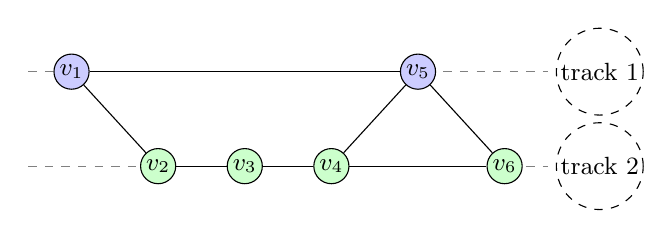
\begin{tikzpicture}[x=1.1cm,y=1.2cm,
    every node/.style={circle,draw,inner sep=1pt,font=\small}]

    % Track lines
    \draw[dashed,gray] (0.5,1.0) -- (6.5,1.0)
      node[right=1mm,black] {$\text{track }1$};
    \draw[dashed,gray] (0.5,0.0) -- (6.5,0.0)
      node[right=1mm,black] {$\text{track }2$};

    % Vertices on track 1
    \node[fill=blue!20]  (v1) at (1,1.0) {$v_1$};
    \node[fill=blue!20]  (v5) at (5,1.0) {$v_5$};

    % Vertices on track 2
    \node[fill=green!20] (v2) at (2,0.0) {$v_2$};
    \node[fill=green!20] (v3) at (3,0.0) {$v_3$};
    \node[fill=green!20] (v4) at (4,0.0) {$v_4$};
    \node[fill=green!20] (v6) at (6,0.0) {$v_6$};

    % Same-track edges
    \draw (v1) -- (v5);                  % track 1
    \draw (v2) -- (v3) -- (v4) -- (v6);  % track 2

    % Cross-track edges
    \draw (v1) -- (v2);
    \draw (v5) -- (v4);
    \draw (v5) -- (v6);

    % % BFS layers from v1
    % \node[above=5mm,align=center,font=\scriptsize] at (1,1.0)
    %   {$L_0=\{v_1\}$};
    % \node[below=4mm,align=center,font=\scriptsize] at (3.5,0.0)
    %   {$L_1=\{v_2,v_5\}$};
    % \node[below=4mm,align=center,font=\scriptsize] at (4.5,0.0)
    %   {$L_2=\{v_3,v_4,v_6\}$};

  \end{tikzpicture}
  \caption{A $2$-track nearest-neighbor graph in which a BFS from $v_1$ has
  $|L_0|=1$, $|L_1|=2$, and $|L_2|=3$.}
  \label{fig:bfs-2-then-3}
\end{figure}

\begin{example}[A $2$-then-$3$ BFS layering in a $2$-track NN graph]
\label{ex:bfs-2-then-3}
Consider the $2$-track layout in Figure~\ref{fig:bfs-2-then-3} with global
order
\[
  v_1 < v_2 < v_3 < v_4 < v_5 < v_6,
\]
track assignment
\[
  \tau(v_1)=\tau(v_5)=1,
  \qquad
  \tau(v_2)=\tau(v_3)=\tau(v_4)=\tau(v_6)=2,
\]
and edges
\[
  \{v_1,v_5\},\;
  \{v_2,v_3\},\;
  \{v_3,v_4\},\;
  \{v_4,v_6\},\;
  \{v_1,v_2\},\;
  \{v_5,v_4\},\;
  \{v_5,v_6\}.
\]
Every edge is between nearest neighbors on some track (either the same track
or the opposite track), so this is a valid $2$-track nearest-neighbor layout.

Run BFS from root $v_1$.  The layers are:
\[
  L_0 = \{v_1\},\quad
  L_1 = \{v_2,v_5\},\quad
  L_2 = \{v_3,v_4,v_6\}.
\]
Indeed:
\begin{itemize}[leftmargin=2em]
  \item From $L_0=\{v_1\}$ we discover its neighbors $v_2$ and $v_5$, so
        $|L_1|=2$.
  \item From $L_1$ we discover, in total, the neighbors $v_3$ (via $v_2$)
        and $v_4,v_6$ (via $v_5$), giving $L_2=\{v_3,v_4,v_6\}$ and
        $|L_2|=3$.
\end{itemize}
Thus this graph exhibits the pattern
\[
  |L_0| = 1,\quad |L_1| = 2,\quad |L_2| = 3
\]
for a perfectly legitimate BFS, contradicting the proposed rule that a
layer of size $3$ cannot be preceded by a layer of size $2$ in any
$2$-track nearest-neighbor graph.
\end{example}

Example~\ref{ex:bfs-2-then-3} shows that such BFS layer-size patterns are
too delicate to use as necessary conditions for $2$-track nearest-neighbor
layouts: even very small graphs that \emph{do} admit such layouts can have
BFS layer sequences of the form $2 \to 3$.  For this reason we abandoned
all BFS-based ``layer-size'' cuts and kept only the robust local structural
conditions (degree bounds, planarity, and the absence of $K_4$) in the main
algorithm.

% =====================================================
\section{Bonus Track: Computing the Exact Track Number $\mathrm{tn}(G)$}
\label{sec:bonus-track}
% =====================================================

We now present a complete algorithm for computing the exact \emph{track number}
$\mathrm{tn}(G)$ of a graph $G$. Recall that $\mathrm{tn}(G)$ is the minimum $k$
such that $G$ admits a nearest-neighbor $k$-track layout. While
Section 9 addressed the recognition problem for $k \le 2$,
here we tackle the general case.

\subsection{Lower bound: degree-based certificate}

\paragraph{Action.}
Given the maximum degree $\Delta(G)$, we compute the immediate lower bound
\[
  k \;\ge\; k_{\min} \;:=\; \left\lceil \frac{\Delta(G)}{2} \right\rceil.
\]

\paragraph{Theoretical justification.}

\begin{proposition}[Degree lower bound]
\label{prop:bonus-degree-lb}
For any graph $G$ with maximum degree $\Delta(G)$,
\[
  \mathrm{tn}(G) \;\ge\; \left\lceil \frac{\Delta(G)}{2} \right\rceil.
\]
\end{proposition}

\begin{proof}
Let $v$ be a vertex of degree $\Delta(G)$ and suppose $G$ admits a
$k$-track layout $(\tau,p)$. Vertex $v$ has at most $2k$ legal neighbors:
on each of the $k$ tracks, at most one predecessor and one successor
(relative to the global order $p$) can be adjacent to $v$. Hence
$\Delta(G) \le 2k$, yielding $k \ge \lceil \Delta(G)/2 \rceil$.
\end{proof}

\subsection{Trivial structures: trees and linear forests}

\paragraph{Action.}
If $G$ is a tree (connected, acyclic), the track number is given exactly by
\[
  \mathrm{tn}(T) \;=\; \left\lceil \frac{\Delta(T)}{2} \right\rceil.
\]
If $G$ is a linear forest (disjoint union of paths), then $\mathrm{tn}(G)=1$.

\paragraph{Theoretical justification.}

\begin{lemma}[Track number for trees]
\label{lem:bonus-trees}
Let $T$ be a tree with maximum degree $\Delta$. Then
$\mathrm{tn}(T) = \lceil \Delta/2 \rceil$.
\end{lemma}

\begin{proof}
The lower bound follows from Proposition~\ref{prop:bonus-degree-lb}. For
the upper bound, we use a DFS-based construction. Root $T$ at an arbitrary
vertex $r$ and perform a depth-first traversal. When visiting a vertex $v$
with children $c_1,\dots,c_d$, assign the children to tracks in a
round-robin fashion: child $c_i$ is placed on track $((i-1) \bmod k)+1$,
where $k = \lceil\Delta/2\rceil$. Place $v$ immediately before its
children in the global order. Since each vertex has at most $\Delta$
neighbors and they are distributed across $k$ tracks, each track receives
at most $\lceil \Delta/k \rceil \le 2$ neighbors of $v$, ensuring all
edges are legal.
\end{proof}

\begin{corollary}
A graph $G$ satisfies $\mathrm{tn}(G)=1$ if and only if $G$ is a linear
forest (disjoint union of paths and isolated vertices).
\end{corollary}

\subsection{Kernelization: leaf pruning}

\paragraph{Action.}
Repeatedly remove all degree-$1$ vertices (leaves) from $G$ until no more
exist. Let $G'$ denote the resulting graph. Then
\[
  \mathrm{tn}(G) \;=\; \max\!\bigl(\mathrm{tn}(G'),\, k_{\min}\bigr),
\]
where $k_{\min}$ was computed from the original $\Delta(G)$.

\paragraph{Theoretical justification.}

\begin{lemma}[Leaf pruning preserves track number]
\label{lem:bonus-leaf-pruning}
Let $v$ be a leaf of $G$ with unique neighbor $u$. Then
\[
  \mathrm{tn}(G) \;=\; \max\!\bigl(\mathrm{tn}(G-v),\,
  \lceil \deg_G(u)/2 \rceil\bigr).
\]
In particular, if $\deg_G(u) \le 2\,\mathrm{tn}(G-v)$, then
$\mathrm{tn}(G) = \mathrm{tn}(G-v)$.
\end{lemma}

\begin{proof}
Any layout of $G$ restricts to a layout of $G-v$, so
$\mathrm{tn}(G-v) \le \mathrm{tn}(G)$. Conversely, given a layout of $G-v$
with $k$ tracks, we can insert $v$ adjacent to $u$ in the global order on
any track where $u$'s predecessor or successor slot is free. Since $u$ has
at most $2k$ legal neighbor slots and uses $\deg_{G-v}(u) < \deg_G(u)$
of them in $G-v$, a free slot exists whenever $k \ge \lceil\deg_G(u)/2\rceil$.
\end{proof}

\subsection{Biconnected component decomposition}

\paragraph{Action.}
Decompose $G'$ into its biconnected components (blocks) $B_1,\dots,B_m$.
Solve each block independently and return
\[
  \mathrm{tn}(G') \;=\; \max_{1 \le i \le m} \mathrm{tn}(B_i).
\]

\paragraph{Theoretical justification.}

\begin{lemma}[Track number from biconnected components]
\label{lem:bonus-biconnected}
Let $B_1,\dots,B_m$ be the biconnected components of a graph $H$. Then
\[
  \mathrm{tn}(H) \;=\; \max_{1 \le i \le m} \mathrm{tn}(B_i).
\]
\end{lemma}

\begin{proof}
The inequality $\mathrm{tn}(H) \ge \max_i \mathrm{tn}(B_i)$ is immediate:
any layout of $H$ restricts to a layout of each $B_i$.

For the reverse inequality, let $k = \max_i \mathrm{tn}(B_i)$. Build a
block-cut tree of $H$. Starting from an arbitrary block $B_1$, fix a
$k$-track layout $(\tau_1,p_1)$ for $B_1$. For each cut vertex $c$
connecting $B_1$ to another block $B_j$, take a $k$-track layout of $B_j$
and translate its global order so that $c$ occupies the same position as
in $B_1$. Since blocks share at most one vertex (the cut vertex), layouts
can be concatenated without conflict. Iterating over the block-cut tree
yields a $k$-track layout for all of $H$.
\end{proof}

\subsection{Exact solver via backtracking}

\paragraph{Action.}
For each block $B_i$ that is neither a tree nor trivial, run a backtracking
search. Starting from $k = k_{\min}$, attempt to construct a valid
$k$-track layout by:
\begin{enumerate}[label=(\alph*)]
  \item Selecting an ordering of vertices (using heuristics: high-degree
        vertices first).
  \item Assigning each vertex to a track and position while checking:
        \begin{itemize}
          \item The degree constraint: no vertex has $>2$ neighbors per track.
          \item The triplet constraint: no forbidden pattern $P^{(1)}$ or $P^{(2)}$.
        \end{itemize}
  \item Backtracking on conflicts; if all orderings fail, increment $k$.
\end{enumerate}

\paragraph{Theoretical justification.}

\begin{theorem}[Correctness of backtracking]
\label{thm:bonus-backtracking}
The backtracking algorithm terminates and returns the exact track number
$\mathrm{tn}(B)$ for any block $B$.
\end{theorem}

\begin{proof}
\emph{Termination:} For any graph on $n$ vertices, $\mathrm{tn}(B) \le n$
(place each vertex on its own track). Thus the search over $k$ is bounded.

\emph{Soundness:} If the algorithm returns $k$, it has found a valid
$k$-track layout satisfying all constraints.

\emph{Completeness:} If a $k$-track layout exists, the backtracking search
explores all orderings and track assignments (up to pruning), so it will
find one.
\end{proof}

\begin{remark}[Pruning strategies]
The search space is reduced by:
\begin{itemize}
  \item \textbf{Degree pruning:} If a partial assignment gives a vertex
        $>2$ neighbors on some track, prune immediately.
  \item \textbf{Symmetry breaking:} Fix the track of the first vertex and
        break ties lexicographically.
  \item \textbf{Lower bound propagation:} If a subgraph requires $k'$
        tracks, prune branches with $k < k'$.
\end{itemize}
\end{remark}

\subsection{Aggregation: final track number}

\paragraph{Action.}
After computing $\mathrm{tn}(B_i)$ for each block, aggregate:
\[
  \mathrm{tn}(G) \;=\; \max\Bigl(k_{\min},\;
  \max_{1 \le i \le m} \mathrm{tn}(B_i)\Bigr).
\]

\paragraph{Theoretical justification.}
This follows directly from Lemma~\ref{lem:bonus-leaf-pruning} (leaf pruning
preserves the bound from $\Delta$) and Lemma~\ref{lem:bonus-biconnected}
(track number is the max over blocks).

\subsection{Complete algorithm and complexity}

\begin{center}
\fbox{\parbox{0.9\textwidth}{
\textbf{Algorithm: Compute $\mathrm{tn}(G)$}
\begin{enumerate}[leftmargin=2em]
  \item \textbf{Input:} Graph $G=(V,E)$.
  \item Compute $k_{\min} := \lceil \Delta(G)/2 \rceil$.
  \item \textbf{If} $G$ is a forest, \textbf{return} $k_{\min}$.
  \item Prune all leaves to obtain $G'$.
  \item Decompose $G'$ into biconnected components $B_1,\dots,B_m$.
  \item \textbf{For each} $B_i$:
    \begin{enumerate}[label=(\alph*)]
      \item If $B_i$ is a single edge or vertex, $\mathrm{tn}(B_i):=1$.
      \item Set $k := \max(\lceil \Delta(B_i)/2 \rceil,\, k_{\max})$.
            \textit{(Skip values $\le k_{\max}$ already ruled out.)}
      \item Run backtracking starting from $k$ to find $\mathrm{tn}(B_i)$.
      \item Update $k_{\max} := \max(k_{\max}, \mathrm{tn}(B_i))$.
    \end{enumerate}
  \item \textbf{Return} $\max(k_{\min}, \max_i \mathrm{tn}(B_i))$.
\end{enumerate}
}}
\end{center}

\paragraph{Complexity analysis.}
\begin{itemize}
  \item Steps 2--5 run in $O(n+m)$ time (linear in the size of $G$).
  \item Step 6 (backtracking) is exponential in the size of each block in
        the worst case, but polynomial for bounded-degree graphs or when
        $k$ is small.
  \item For practical graphs (sparse, low degree), the algorithm often
        terminates quickly due to aggressive pruning.
  \item \textbf{Empirical observation:} In practice, most graphs satisfy
        $\mathrm{tn}(G) \le \lceil \Delta(G)/2 \rceil + 1$, so the solver
        rarely needs to test more than two values of $k$ per block.
\end{itemize}

\begin{remark}[Relation to Linear Arboricity]
The \emph{linear arboricity} $\mathrm{la}(G)$ is the minimum number of linear
forests needed to cover all edges of $G$. The Akiyama--Chv\'{a}tal Conjecture
states that $\mathrm{la}(G) \le \lceil (\Delta(G)+1)/2 \rceil$ for every graph
(it is known that $\mathrm{la}(G) \ge \lceil \Delta(G)/2 \rceil$).
However, the \emph{track number} $\mathrm{tn}(G)$ is a different problem: it
requires all linear forests to share a \emph{single global vertex ordering},
which may force $\mathrm{tn}(G) > \mathrm{la}(G)$. The exact relationship
between these invariants remains an open problem.
\end{remark}

\begin{remark}[Relation to NP-hardness]
Determining whether $\mathrm{tn}(G) \le k$ is NP-complete for general $k$
(it generalizes graph coloring-like constraints). However, for fixed $k$,
the problem is in P: one can enumerate all $k^n \cdot n!$ possible layouts
in time $O((k \cdot n)^{O(1)} \cdot k^n \cdot n!)$, which is constant for
fixed $k$. Our backtracking approach with pruning makes this tractable for
small $k$ and moderate $n$.
\end{remark}

\end{document}
